\RequirePackage{plautopatch}
\documentclass[report,a4paper,uplatex,dvipdfmx,11pt]{jsbook}
\usepackage[dvipdfmx]{graphicx,color}
\usepackage{amsmath, amssymb,  latexsym, mathtools}
\usepackage{amsthm}
\usepackage{amsfonts}
\usepackage{bm} %数式中でボールド体も斜体にする。\bm{a}と書けば、斜体ボールドのaが書ける
\usepackage{midpage}
\usepackage[dvipdfmx]{graphicx,color}
\usepackage[hyphens]{url}
\usepackage[sort,compress,numbers]{natbib} % apsrev4-2ja.bstを使うのに必要
\usepackage{doi}
\usepackage{cleveref}
\usepackage{tocloft}
\usepackage{autonum}
\usepackage{hyperref}
\usepackage{pxjahyper}
\usepackage{xcolor}
\hypersetup{
  colorlinks=true,
  bookmarksnumbered=true,
  citecolor=blue,
  linkcolor=violet,
  urlcolor=blue,
  }

\newtheoremstyle{myDefinition}%   % スタイル名
    {11pt}%b                     % 上部スペース
    {16pt}%                      % 下部スペース
    {}%              % 本文フォント
    {}%                      % 1行目のインデント量
    {\bfseries}%             % 見出しフォント
    {.}%                     % 見出し後の句読点
    {11pt}%                     % 見出し後のスペース
    {\thmname{#1}\thmnumber{ #2}\thmnote{ (#3)}}

\theoremstyle{myDefinition}
\newtheorem{definition}{Definition}[section]
\theoremstyle{myDefinition}
\newtheorem{theorem}[definition] {Theorem}
\theoremstyle{myDefinition}
\newtheorem{proposition}[definition] {Proposition}
\theoremstyle{myDefinition}
\newtheorem{lemma}[definition] {Lemma}
\theoremstyle{myDefinition}
\newtheorem{corollary}[definition] {Corollary}
\theoremstyle{myDefinition}
\newtheorem{example}[definition] {Example}
\theoremstyle{myDefinition}
\newtheorem{remark}[definition] {Remark}

\crefname{definition}{}{}
\crefname{example}{}{}
\crefname{theorem}{}{}
\crefname{lemma}{}{}
\crefname{corollary}{}{}
\crefname{remark}{}{}
\crefname{proposition}{}{}
\crefname{proof}{}{}
\crefname{figure}{}{}
\crefname{chapter}{}{}
\crefname{section}{}{}
\crefname{subsection}{}{}
\crefname{equation}{式}{式}

\creflabelformat{definition}{#2\textbf{Definition} \textbf{#1}\textbf{.}#3}
\creflabelformat{example}{#2\textbf{Example} \textbf{#1}\textbf{.}#3}
\creflabelformat{theorem}{#2\textbf{Theorem} \textbf{#1}\textbf{.}#3}
\creflabelformat{lemma}{#2\textbf{Lemma} \textbf{#1}\textbf{.}#3}
\creflabelformat{corollary}{#2\textbf{Corollary} \textbf{#1}\textbf{.}#3}
\creflabelformat{remark}{#2\textbf{Remark} \textbf{#1}\textbf{.}#3}
\creflabelformat{proposition}{#2\textbf{Proposition} \textbf{#1}\textbf{.}#3}
\creflabelformat{proof}{#2\textit{Proof} \textbf{#1}#3}
\creflabelformat{figure}{#2Figure #1#3}
\creflabelformat{chapter}{#2第#1章#3}
\creflabelformat{section}{#2第#1節#3}
\creflabelformat{subsection}{#2第#1小節#3}

\renewcommand{\figurename}{Figure }
\def\jaitalic#1{\makebox[2.25zw][l]{\vphantom{#1}\rotatebox{-48.8}{\scalebox{0.875}[1.143]{\rotatebox{41.2}{\smash{\rlap{#1}}}}}}}


% 参考文献の書式の設定-----------------------------------------------------------------
% \bibliographystyle{apsrev4-2ja} % アメリカ物理学会(APS)の標準のbibtexスタイルファイル
% \bibliographystyle{junsrt} % 文献のタイトルまで表示したい場合はこちらを使う
% \bibliographystyle{jplain}
\bibliographystyle{amsplain}
% -------------------------------------------------------------------------------------


% 余白の設定をするためのパッケージ------------------------------
%\usepackage[pass]{geometry}
%\usepackage{bxpapersize}
% --------------------------------------------------------------


% 章見出しの上の余白を小さくする--------------------------------
\usepackage{etoolbox}
\makeatletter
\patchcmd{\@makechapterhead}{\vspace*{2\Cvs}}{}{}{}
\patchcmd{\@makeschapterhead}{\vspace*{2\Cvs}}{}{}{}
\makeatother
\renewcommand{\cftbeforetoctitleskip}{0pt}
% --------------------------------------------------------------


% 目次のフォントについて----------------------------------------------------
% 1. 見出しの文字を明朝体にする(太字にはならない)
%\renewcommand{\headfont}{\mcfamily}

% 2. 明朝体の太字を使う場合は、
%\usepackage[deluxe]{otf}
%\renewcommand{\headfont}{\mcfamily\bfseries}

% 3. 見出し全てではなく、目次のフォントのみ変更する場合は、
\renewcommand{\cftchapnumwidth}{3.8em}
\renewcommand{\cftchapfont}{\mcfamily}
\renewcommand{\cftchappagefont}{\rmfamily}
% --------------------------------------------------------------------------


% 目次に参考文献を表示する ---------------------------------------
\makeatletter
\renewenvironment{thebibliography}[1]{%
 \bibsection\parindent \z@\bibpreamble\bibfont\list
   {\@biblabel{\arabic{NAT@ctr}}}{\@bibsetup{#1}%
   \addcontentsline{toc}{chapter}{\bibname}%
    \setcounter{NAT@ctr}{0}}%
    \ifNAT@openbib
      \renewcommand\newblock{\par}
    \else
      \renewcommand\newblock{\hskip .11em \@plus.33em \@minus.07em}%
    \fi
    \sloppy\clubpenalty4000\widowpenalty4000
    \sfcode`\.=1000\relax
    \let\citeN\cite \let\shortcite\cite
    \let\citeasnoun\cite
 }{\def\@noitemerr{%
  \PackageWarning{natbib}
     {Empty `thebibliography' environment}}%
  \endlist\vskip-\lastskip}
 \let\bibfont\relax
\makeatother
% ----------------------------------------------------------------


% 卒論で、図をページ数に含めたくないときに用いる図・表環境-------------
\newenvironment{clearpagefigure}
{\newpage
  \begin{midpage}
  \begin{figure}[htbp]
  \centering
  \thispagestyle{empty}
  \addtocounter{page}{-1}}
{\end{figure}
  \end{midpage}
  \newpage}

\newenvironment{clearpagetable}
{
\clearpage
\begin{table}
\centering
\thispagestyle{empty}
\addtocounter{page}{-1}
}
{\end{table}}
% ---------------------------------------------------------------------


\setcounter{tocdepth}{2} % 目次にどのレベルのセクションまで反映させるか。2だとsubsectionまで。

\allowdisplaybreaks % 数式の途中での改ページを許す

%---------------------------------------------



\title{パズルルールの自動作成を目指した数学的考察}
\author{前田樹}
\date{\today}

\begin{document}

\maketitle

\frontmatter
\chapter*{{\rm \bf Abstract}}\label{chapter:Abstract}
最適化を好む現代社会においては, エンターテイメントもその対象である. 技術の発展とともに, 人々は冗長なエンターテイメントを忌避するようになり, より短く, より楽しく, より強い刺激を求めるようになった. 無駄を徹底的に省いた娯楽に私はどこかもの寂しさを感じずにはいられない. 私たちが幼少期の頃に触れた娯楽は, 無駄の多い, 冗長なものばかりだった. そうすることでしか得られないカタルシスがあったのだろう. その媒体が私にとってはパズルだった. だが, パズルは時代の波に追いやられ, いまや本屋の棚の片隅で存在感を希薄にしているのである. ただ, 私は面白いパズルがもう一度解きたい. その一心で, 私自身が新しいパズルルールを生み出し, 自分の手で面白いパズルを解くことを叶えるために本研究を着想した.

% パズルは, 世界中で多くの人々を魅了する娯楽の一つである. その形態は多岐にわたり, 様々なパズルが研究対象となっている. パズルの一つであるペンシルパズルは, 世界で最も人気のパズルジャンルのうちの一つである. ペンシルパズルは完全情報確定パズルと言われるものの一種であり, その計算量や解法アルゴリズム, あるいは問題の自動作成等については深く研究が進んでいる. しかし一つ抽象度を上げた, ペンシルパズルのパズルルールを自動的に作成したという先行研究は現時点で存在しない. 先行研究で確認されているように, 商業用ゲームでのマンネリ化を解消するためにはパズルが有効である. しかし, 一種類のパズルのみではマンネリ化を解消することは難しく, 生産コストの点から多種多様なパズルルールを生み出すことは難しい. そこで, パズルルールを自動作成することが求められている.

本研究の目標は, パズルルールの自動作成に関する理論の確立と実践である. この世に知られていないパズルルールを自動的に無際限に, 心の欲するところに従うままに, 生み出すことである. そこで, パズルルールの自動作成にあたり, ペンシルパズルに着目し, パズルルールの自動作成に関する研究を調査した. 驚くことに, パズルを扱う応用数学やゲーム開発などの関連分野において, そのような観点からの先行研究は全く見当たらず, おそらくはも存在しないと考えられた. この原因には, ペンシルパズルのパズルルールに関し, 統一的な数学的記述の整理がなされておらず, 自動生成はもとより, パズルルールの体系化を行うための数学的な道具も用意されていないことが分かった. そこで, 本研究の目的はパズルルールを数学的に定義し, それらにまつわる概念を整理することとした.

そこで本論文ではパズルルールにまつわる基礎的な概念として, 平面グリッドにおいて位置, 状態, 盤面などと数学的に定義した上で, パズルルールを記述するために四つの概念を導入した(\textit{codomain}, \textit{conditions}, \textit{Hidden Information}(HI), \textit{identification}). そして, それらの概念の組み合わせでパズルルールが数学的に定義できることを主張した. また, それらの数学的記述の妥当性を検証するために\cref{chapter:Demonstration}ではそれらを用いて既存のパズルルールを数学的に記述できることを実証した. さらに本研究の定義を用いて新しいパズルルールを作成し, そのパズルルールの問題が実際に存在することも示した.

本研究でのパズルルールの数学的な記述を用いることにより, 既存のパズルルールがどのような性質を持っているかの体系的な整理が期待される. また, その性質を分類, 抽象化することにより, それらの性質を持った新規のパズルルールを機械的に作成することが期待される. また, 先行研究の定理を本研究に適用できる制約条件を明確にすることで, 将来的に自動作成されたパズルルールから具体的なパズルの問題を自動作成も期待される. さらに, ペンシルパズルのパズルルール自体の難易度評価がなされた先行研究は存在しない. そこで, 本研究のパズルルールの数学的な記述を行うことにより, パズルルール自体の難易度評価の可能性についても説明した.
\tableofcontents

\mainmatter
\chapter{緒言}
\section{研究背景}
本研究は
\section{研究目的}

\chapter{準備}\label{chapter:Prepare}
\section{章の概略}\label{section:Outline}
この章では準備としてペンシルパズルに関わる用語の定義を行う. ただし, ペンシルパズルとは「サイズ$m\times n$の平面グリッドを与えたとき, パズルルールに定められた条件と, その解答ステップにおいて明らかになっている解から格子点, 細胞, 辺のいずれかの未知情報に論理的推測から解を書き込み, 全ての格子点, 細胞, 辺がパズルルールに定められた条件を満たす完成盤面へと解く行為と, その問題やルールなどを一括りに呼ぶ概念」とし, 明確な定義は行わずあくまで概念として以下もペンシルパズルという用語を使用する. ただし, 格子点, 細胞, 辺というのは\cref{fig:Board}で与える図中の名前とそれぞれ対応させるものとする.
ペンシルパズルは, 例としてナンバープレイス(\cref{fig:SamplePuzzle})などが与えられる.
\cref{section:WordDefinition}ではペンシルパズルで与えられる盤面と, それに付随する用語を定義する.
\cref{section:MathematicalDefinition}ではペンシルパズルにおける, 諸概念の数学的な定義を行う.
\cref{section:RelationDefinition}では\cref{section:MathematicalDefinition}で定義する変数同士の関係性についての定義を行う.
\cref{section:GraphDefinition}ではペンシルパズルにおいて考えられるグラフという概念の定義を行う.

\section{用語の定義}\label{section:WordDefinition}
この節ではペンシルパズルにおける用語を定義する. ただし, ペンシルパズルとは「サイズ$m\times n$の平面グリッドを与えたとき, 格子点, 細胞, 辺のいずれかの未知情報に対し, パズルルールに定められた条件とその解答ステップにおいて明らかになっている既知情報から一意に定まる解を書き込み, 全ての格子点, 細胞, 辺がパズルルールに定められた条件を満たす完成盤面へと解く行為と, その問題やルールなどを一括りに呼ぶ概念」とし, 明確な定義は行わずあくまで概念として以下もペンシルパズルという用語を使用する. ただし, 格子点, 細胞, 辺は\cref{fig:Board}で与える図中の名前とそれぞれ対応させるものとし, ある解答ステップにおける既知情報とはあるパズルの問題があったときの初期状態と, それまでの解答ステップにより得られた解のことを指すものとする. ペンシルパズルは, 例としてナンバープレイス(\cref{fig:SamplePuzzle})などが与えられる.

以下の説明のために盤面, 完成盤面, 未完成盤面を定義する. \cref{fig:Board}で与えたようなグリッドに対し, 各格子点, 細胞, 辺に対応する解が存在するものを総称して\textgt{盤面}と定義する. しかし, その解が未知, 既知に関わらず盤面と呼ぶ. ただし解とはペンシルパズルにおいて格子点, 細胞, 辺に対して写像で送った際に数値や, 変数のことである. \cref{fig:SamplePuzzle}に与えたパズルでは, 左上端の細胞の解が2に対応し, 右下端の細胞の解は未知である(既知の場合3).
また, 全ての格子点, 細胞, 辺の解がパズルルールに定められた条件を満たしている盤面のことを\textgt{完成盤面}と定義する. さらに任意の格子点, 細胞, 辺の解が未知であるものが存在する盤面の中で, 解を既知にしたときに対応する完成盤面がただ一つしかない盤面を\textgt{未完成盤面}と定義する. 未完成盤面と完成盤面の例として\cref{fig:SamplePuzzle}を与える. 図中左が未完成盤面, 図中右が完成盤面である.

上の記述より, 一つの完成盤面には複数の未完成盤面が対応する(一つの操作(未知情報に解を書き込む)を課した未完成盤面もまた未完成盤面. ).このとき, その複数の未完成盤面と, 完成盤面の集合全体をパズルルールの\textgt{問題}と定義する.

\begin{clearpagefigure}

  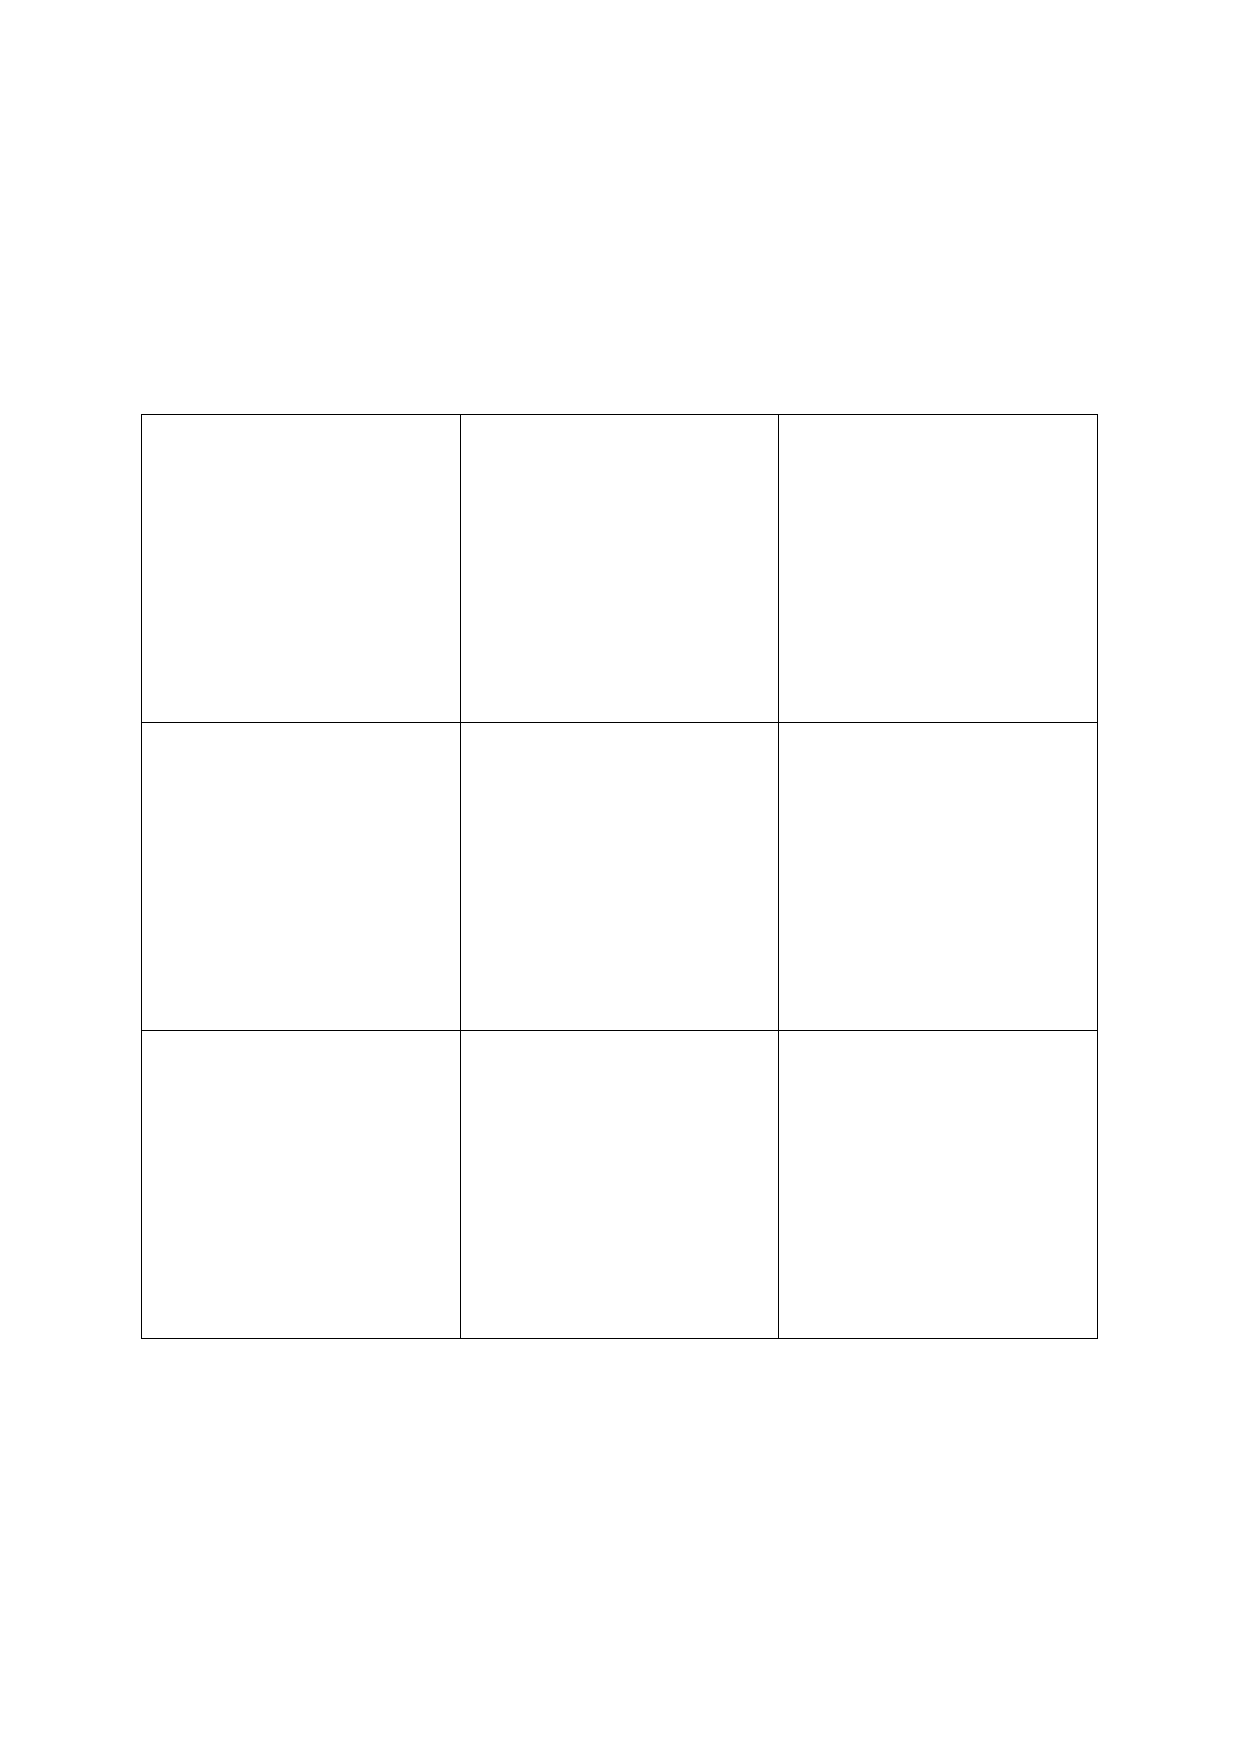
\includegraphics[width=8cm,clip]{fig/board.png}
  \caption{}
  \label{fig:Board}
\end{clearpagefigure}

\begin{clearpagefigure}
  \includegraphics[width=8cm,clip]{fig/samplePuzzle.png}
  \caption{}
  \label{fig:SamplePuzzle}
\end{clearpagefigure}

\section{盤面上の情報に関する概念の数学的定義}\label{section:MathematicalDefinition}
この節ではペンシルパズルにおける盤面上の情報に関する各概念を数学的に定義する. ここで定義するものは全て直感的な定義と違わないように行う.
平面グリッドを与えたとき, ペンシルパズルの盤面には左上から各格子点に対し座標$(i,j)$を割り振ることができる(\cref{fig:Coordinate}). そうしたとき, グリッドにおける格子点, 細胞, 辺に対して\cref{fig:VariableAtBoard}で表されるように変数を与えることができる.
これをそれぞれ数学的に格子点$p(i,j)$, 細胞$c(i,j)$, 横辺$h(i,j)$, 縦辺$v(i,j)$として定義する.

\begin{clearpagefigure}
  \includegraphics[width=8cm,clip]{fig/coordinate.png}
  \caption{}
  \label{fig:Coordinate}
\end{clearpagefigure}

\begin{definition}[格子点$p(i,j)$, 細胞$c(i,j)$, 横辺$h(i,j)$, 縦辺$v(i,j)$]\label{definition:VariableAtBoard}
  \textgt{格子点}$p(i,j)$($(i,j)\in \mathbb{Z}^2$)を
  \begin{equation*}
    p(i,j)\coloneqq \{(i,j)\} \quad (1\leq i \leq n, 1\leq j \leq n)
  \end{equation*}
  と定義する.

  以下同様に\textgt{細胞}$c(i,j)$, \textgt{横辺}$h(i,j)$, \textgt{縦辺}$v(i,j)$を
  \begin{gather*}
    c(i,j)\coloneqq  \{(i,j), (i,j+1), (i+1,j), (i+1,j+1)\}  (1\leq i \leq n-1, 1\leq j \leq n-1)  \\
    h(i,j)\coloneqq  \{(i,j), (i,j+1)\}                      (1\leq i \leq n-1, 1\leq j \leq n)    \\
    v(i,j)\coloneqq  \{(i,j), (i+1,j)\}                      (1\leq i \leq n, 1\leq j \leq n-1)
  \end{gather*}
  と定義する.

  ただし, $h(i,j),v(i,j)$の詳細に興味がない場合は, 任意の辺という意味で辺$e(i,j,y)$を
  \begin{equation*}
    e(i,j,y) \coloneqq \{h(1,1),h(1,2),...,h(n-1,n),v(1,1),v(1,2),...,v(n,n-1)\}\ni \forall x \quad (y \in \{h,v\})
  \end{equation*}
  と定義する.
  ただし, $y=h$のとき$e(i,j,h)$は縦辺, $y=v$のとき$e(i,j,v)$は横辺を指すものとする. $(i,j)$の範囲はyによって指定されるそれぞれの変数によって定義されるものとする($y=h$のときは$1\leq i \leq n-1,1\leq j \leq n$).

  また, 格子点, 細胞, 辺の集合の詳細そのものに興味がない場合は任意の格子点, 細胞, 辺という意味で$\lambda(i,j,y)$を
  \begin{equation*}
    \lambda(i,j,y) \coloneqq \{p(i,j),c(i,j),h(i,j),v(i,j)\}\ni \forall x \quad (y \in \{p,c,h,v\})
  \end{equation*}
  と定義する.ただし, $y=p$のときは$\lambda(i,j,p)$は格子点, $y=c$のときは$\lambda(i,j,c)$は細胞, $y=h$のときは$\lambda(i,j,h)$は縦辺, $y=v$のときは$\lambda(i,j,v)$は横辺を指すものとする. $(i,j)$の範囲はyによって指定されるそれぞれの変数によって定義されるものとする($y=p$のときは$1\leq i \leq n,1\leq j \leq n$).
\end{definition}
これら添え字付きの変数を改めて格子点, 細胞, 辺と呼び, これらをまとめた総称として\textgt{盤面上の変数}と呼ぶこととする.

\begin{clearpagefigure}
  \includegraphics[width=8cm,clip]{fig/define.png}
  \caption{}
  \label{fig:VariableAtBoard}
\end{clearpagefigure}

ペンシルパズルにおいて, ソルバーは盤面上の変数に対して解を書き込むことが前提であった(\cref{section:Outline}).解とは, 盤面上の変数に対応して与えられる数値や, 変数のことを指すものとする.
そのため, パズルルールを定義するためには, 解がどのような集合の元に含まれるかを定義する必要がある. そのために以下で\textit{codomain}という用語を用いて解集合を定義する.

\begin{definition}[\textit{codomain}]\label{definition:Codomain}
  盤面上の変数に対し一対一に対応する解が含まれる集合のことを\textbf{\textit{codomain}}と定義する. 格子点, 細胞, 辺の\textit{codomain}を表す集合として$\mathbb{P},\mathbb{C},\mathbb{H},\mathbb{V}$を用いる. $\mathbb{H},\mathbb{V}$の\textit{codomain}が一致している場合にはまとめて$\mathbb{E}$と記述する. \textit{codomain}の詳細に興味がなく, \textit{codomain}全体を考えるときにはそれら集合を含意するものとして$\Lambda$を使用する.
\end{definition}

ここで, 盤面上の変数に対してそれぞれ解として具体的な値(1や3などの数値, あるいは$x_1$などの記号)が対応するがその解は列をなしていて同一の値が含んだ列となることがある.
よって\textit{codomain}と解の列は同一視できないことに注意する. また, パズルルールによっては格子点, 細胞, 辺に解を与えられない場合があり, そのときに限っては\textit{codomain}は$\emptyset$と記述し, 盤面上の変数に対応する解が存在しないことを表すこととする.以下に既存のパズルルールのスリザーリンクを例として用いる. ただし, スリザーリンクのパズルルールは以下のものである. \cite{web:SlitherLink}

\begin{enumerate}
  \item 点と点の間にタテヨコに線を引き, 全体で1つの輪っかを作りましょう.
  \item 4つの点で作られた正方形の中にある数字は, その正方形の辺に引く線の数を表しています. 数字のない正方形には, 何本の線を引くかわかりません.
  \item 線を交差させたり, 枝分かれさせたりしてはいけません.
\end{enumerate}

\begin{clearpagefigure}
  \includegraphics[width=5cm]{fig/slitherlink.png}
  \caption{スリザーリンクの完成盤面}
\end{clearpagefigure}

\begin{example}[スリザーリンクの\textit{codomain}]\label{example:SlitherLinkCodomain}
  スリザーリンクにおいては, \textit{codomain}は以下のように表すことができる. しかし辺が「書かれている」時は1,「書かれていない」時は0に対応させるものとする.
  \begin{gather*}
    \mathbb{P}  =  \emptyset     \\
    \mathbb{C}  =  \{0,1,2,3,4\} \\
    \mathbb{E}  =  \{0,1\}
  \end{gather*}
\end{example}
以上のように\textit{codomain}を考えることにより, 盤面上の変数が含まれる各集合から, \textit{codomain}に送る写像を考えることができる.
\begin{definition}[写像$\bm{p}$, $\bm{c}$, $\bm{h}$, $\bm{v}$]\label{definition:Mapping}
  格子点$p(i,j)$を過不足なくふくむ集合$\{p(i,j)\}$から$\mathbb{P}$に送る写像$\bm{p}$を
  \begin{equation*}
    \begin{array}{rccc}
      \bm{p}\colon & \{p(i,j)\} & \longrightarrow & \mathbb{P} \\
                   & p(i,j)     & \longmapsto     & p_{i,j}
    \end{array}
  \end{equation*}
  と定義する.
  以下同様に$\bm{c}$, $\bm{h}$, $\bm{v}$を

  \begin{equation*}
    \begin{array}{rccc}
      \bm{c}\colon & \{c(i,j)\} & \longrightarrow & \mathbb{C} \\
                   & c(i,j)     & \longmapsto     & c_{i,j}
    \end{array}
  \end{equation*}
  \begin{equation*}
    \begin{array}{rccc}
      \bm{h}\colon & \{h(i,j)\} & \longrightarrow & \mathbb{H} \\
                   & h(i,j)     & \longmapsto     & h_{i,j}
    \end{array}
  \end{equation*}
  \begin{equation*}
    \begin{array}{rccc}
      \bm{v}\colon & \{v(i,j)\} & \longrightarrow & \mathbb{V} \\
                   & v(i,j)     & \longmapsto     & v_{i,j}
    \end{array}
  \end{equation*}
  と定義する.

  ただし, $\bm{h},\bm{v}$の詳細に興味がない場合は, 同様に
  \begin{equation*}
    \begin{array}{rccc}
      \bm{e}\colon & \{e(i,j,y)\} & \longrightarrow & \mathbb{E} \\
                   & e(i,j,y)     & \longmapsto     & e_{i,j,y}
    \end{array}
  \end{equation*}
  と記述し, 上記の写像の詳細に興味がない場合それらの写像全てを含意するものとして$\bm{\lambda}$を用いて
  \begin{equation*}
    \begin{array}{rccc}
      \bm{\lambda}\colon & \{\lambda(i,j,y)\} & \longrightarrow & \Lambda         \\
                         & \lambda(i,j,y)     & \longmapsto     & \lambda_{i,j,y}
    \end{array}
  \end{equation*}
  と記述する.
\end{definition}
集合論の用語を用いると, 解の列$\{\lambda_{1,1,y_{(1,1)}}, \lambda_{1,2,y_{(1,2)}},...\}$と写像$\bm{\lambda}\colon \{\lambda(i,j,y)\} \longrightarrow \Lambda$の間には$\bm{\lambda}(\lambda(i,j,y))=\lambda_{i,j,y}$という自然な一対一対応が存在する.
ここで$\{\lambda_{i,j,y}\}$は$\{\lambda_{1,1,y_{(1,1)}}, \lambda_{1,2,y_{(1,2)}},...\}$であり, 写像$\bm{\lambda}$は$\{\lambda(i,j,y)\}$によって添え字付けられた族である. またこのとき, $\{\lambda(i,j,y)\}$は添字集合で, $\lambda(i,j,y)$はこの写像の添字である.

盤面上の変数とその解(\textit{codomain}の元)の対応は(\cref{definition:Mapping})のように添字によってラベル付けされ, 解同士の関係は(\cref{definition:Codomain})直後で記述したように実際に取る値の如何に関わらず別物として扱う.
盤面上の変数と, その解(\cref{definition:Mapping})との対応が全て分かっているとき, 写像はそれらの取る値を全て列として記述すれば$\bm{\lambda}\Leftrightarrow \{\lambda_{i,j,y}\}$と同一視することができる.

このような種々の定義を導入することにより, $\mathbb{P},\mathbb{C},\mathbb{E}$を与えたとき任意の盤面は
\begin{equation}\label{equation:U}
  U=\Bigl\{\{\bm{p},\bm{c},\bm{e}\}_x\Bigr\}=\biggl\{\Bigl\{\{p_{i,j}\}_x,\{c_{i,j}\}_x,\{e_{i,j,y}\}_x\Bigr\}_x\biggr\} \quad (1\leq x \leq |U|)
\end{equation}
なる集合の一つの元と言うことが出来る.
ただし, 写像$\bm{c}$などは各盤面においてただ一つ存在するものだから, ある具体的な盤面は$\{\bm{p},\bm{c},\bm{e}\}_x$, あるいは$\Bigl\{\{p_{i,j}\}_x,\{c_{i,j}\}_x,\{e_{i,j,y}\}_x\Bigr\}_x$と記述されることに注意する.
また, $\lambda(i,j,y)$が$\lambda_{i,j,y}$と一対一対応することより誤解の恐れがない場合は$\lambda(i,j,y) \in B  $,  $\lambda_{i,j,y}\in B $と記述する.
このときは$B$は集合として$B=\{\lambda(i,j,y)\}_x$を考え, $\lambda_{i,j,y}$も$\bm{\lambda}$によりBの元として扱うこととする.
ただし前と同様$\{\lambda(i,j,y)\}_x$とは$\{\lambda(1,1,y_{(1,1)}), \lambda_(1,2,y_{(1,2)}),...\}$を指すものとする.

ここで, ある問題を与えたとき完成盤面が満たしているべきパズルルールによって定められた条件は, そのまま\cref{equation:U}に条件として記述することができて, これを\textit{conditions}と定義する.
\begin{definition}[\textit{conditions}]\label{definition:Conditions}
  完成盤面において解が満たしているべき必要十分条件のことを\textbf{\textit{conditions}}と定義する.
\end{definition}
\textit{conditions}の具体例は\cref{section:GraphDefinition}で定義するグラフと\cref{definition:Function}で定義する関数を用いる必要があるため, 後の\cref{example:SlitherLinkConditions}で取り上げることとする.

上の\textit{conditions}を用いればあるパズルルールが存在したとき, 完成盤面全体の集合$X$は
\begin{equation}\label{equation:X}
  X=\biggl\{\Bigl\{\{p_{ij}\}_x,\{c_{ij}\}_x,\{e_{i,j,y}\}_x\Bigr\}_x\mid \rm{\textit{conditions}}\biggr\}
\end{equation}
と記述することができる. ベン図は\cref{fig:VennDiagram}のようになる.

\begin{clearpagefigure}
  \includegraphics[width=8cm,clip]{fig/vennDiagram.png}
  \caption{}
  \label{fig:VennDiagram}
\end{clearpagefigure}

\cref{equation:X}で定義した完成盤面から問題へと派生させるために「ソルバーに隠す盤面上の変数の解」として\textit{HI(Hidden Information)}を定義する.
ただし, 「隠す」という言葉は\textit{codomain}から\textit{codomain}に\textit{null}を加えた集合$\Lambda'=\Lambda\cup \textit{null}$への写像$\phi\colon \Lambda \longrightarrow \Lambda'$を解の列に作用させることを意味することとする.
ただし, 解が未知であることを状態として\textbf{\textit{null}}と定義し, 盤面上の変数に対応する解が未知であるときに限り$p_{i,j}=\textit{null}$などとするとする.

ただし, パズルルールによっては解が未知である状態がソルバーに実際に示される数値あるいは変数が\textit{codomain}に含まれる場合があることに注意する. (スリザーリンク(\cref{example:SlitherLinkCodomain})においては$h_{i,j}, v_{i,j} = 0$のとき解が未知である, あるいは解として0を持つことがソルバーに同一の状態として伝えられる. )

\begin{definition}[\textit{HI(Hidden Information)}]\label{definition:HiddenInformation}
  ソルバーから隠す盤面上の変数の部分集合に対応する解の部分列を\textbf{\textit{HI(Hidden Information)}}と定義する.
  ただし, その部分集合はパズルルールによってそれが一意に定まるものではなく問題に依存するものとし, パズルルールでは$\{c_{i,j}\}$と$\{e_{i,j,y}\}$の部分列といったように隠す列及び部分列の情報のみを指定し, 詳細は指定しないものとする.
\end{definition}

\begin{example}[スリザーリンクの\textit{HI}]
  \begin{gather*}
    \{c_{i,j}\}の部分列 \\
    \{e_{i,j,y}\}
  \end{gather*}
\end{example}

完成盤面においては盤面上の変数と解が一対一に対応することにより, $\mathbb{E}$が要素として数値のみを持つ場合に限り新たに下記のような関数を導入することができる(\cref{fig:cross}, \cref{fig:cycle}).

\begin{definition}[\textit{cross}, \textit{cycle}]\label{definition:Function}
  \begin{gather*}
    \textit{cross}(p(i,j))\coloneqq h_{i,j-1}+v_{i-1,j}+h_{i,j}+v_{i,j} \\
    \textit{cycle}(c(i,j))\coloneqq h_{i,j}+v_{i,j}+h_{i+1,j}+v_{i,j+1}
  \end{gather*}
\end{definition}
\begin{clearpagefigure}
  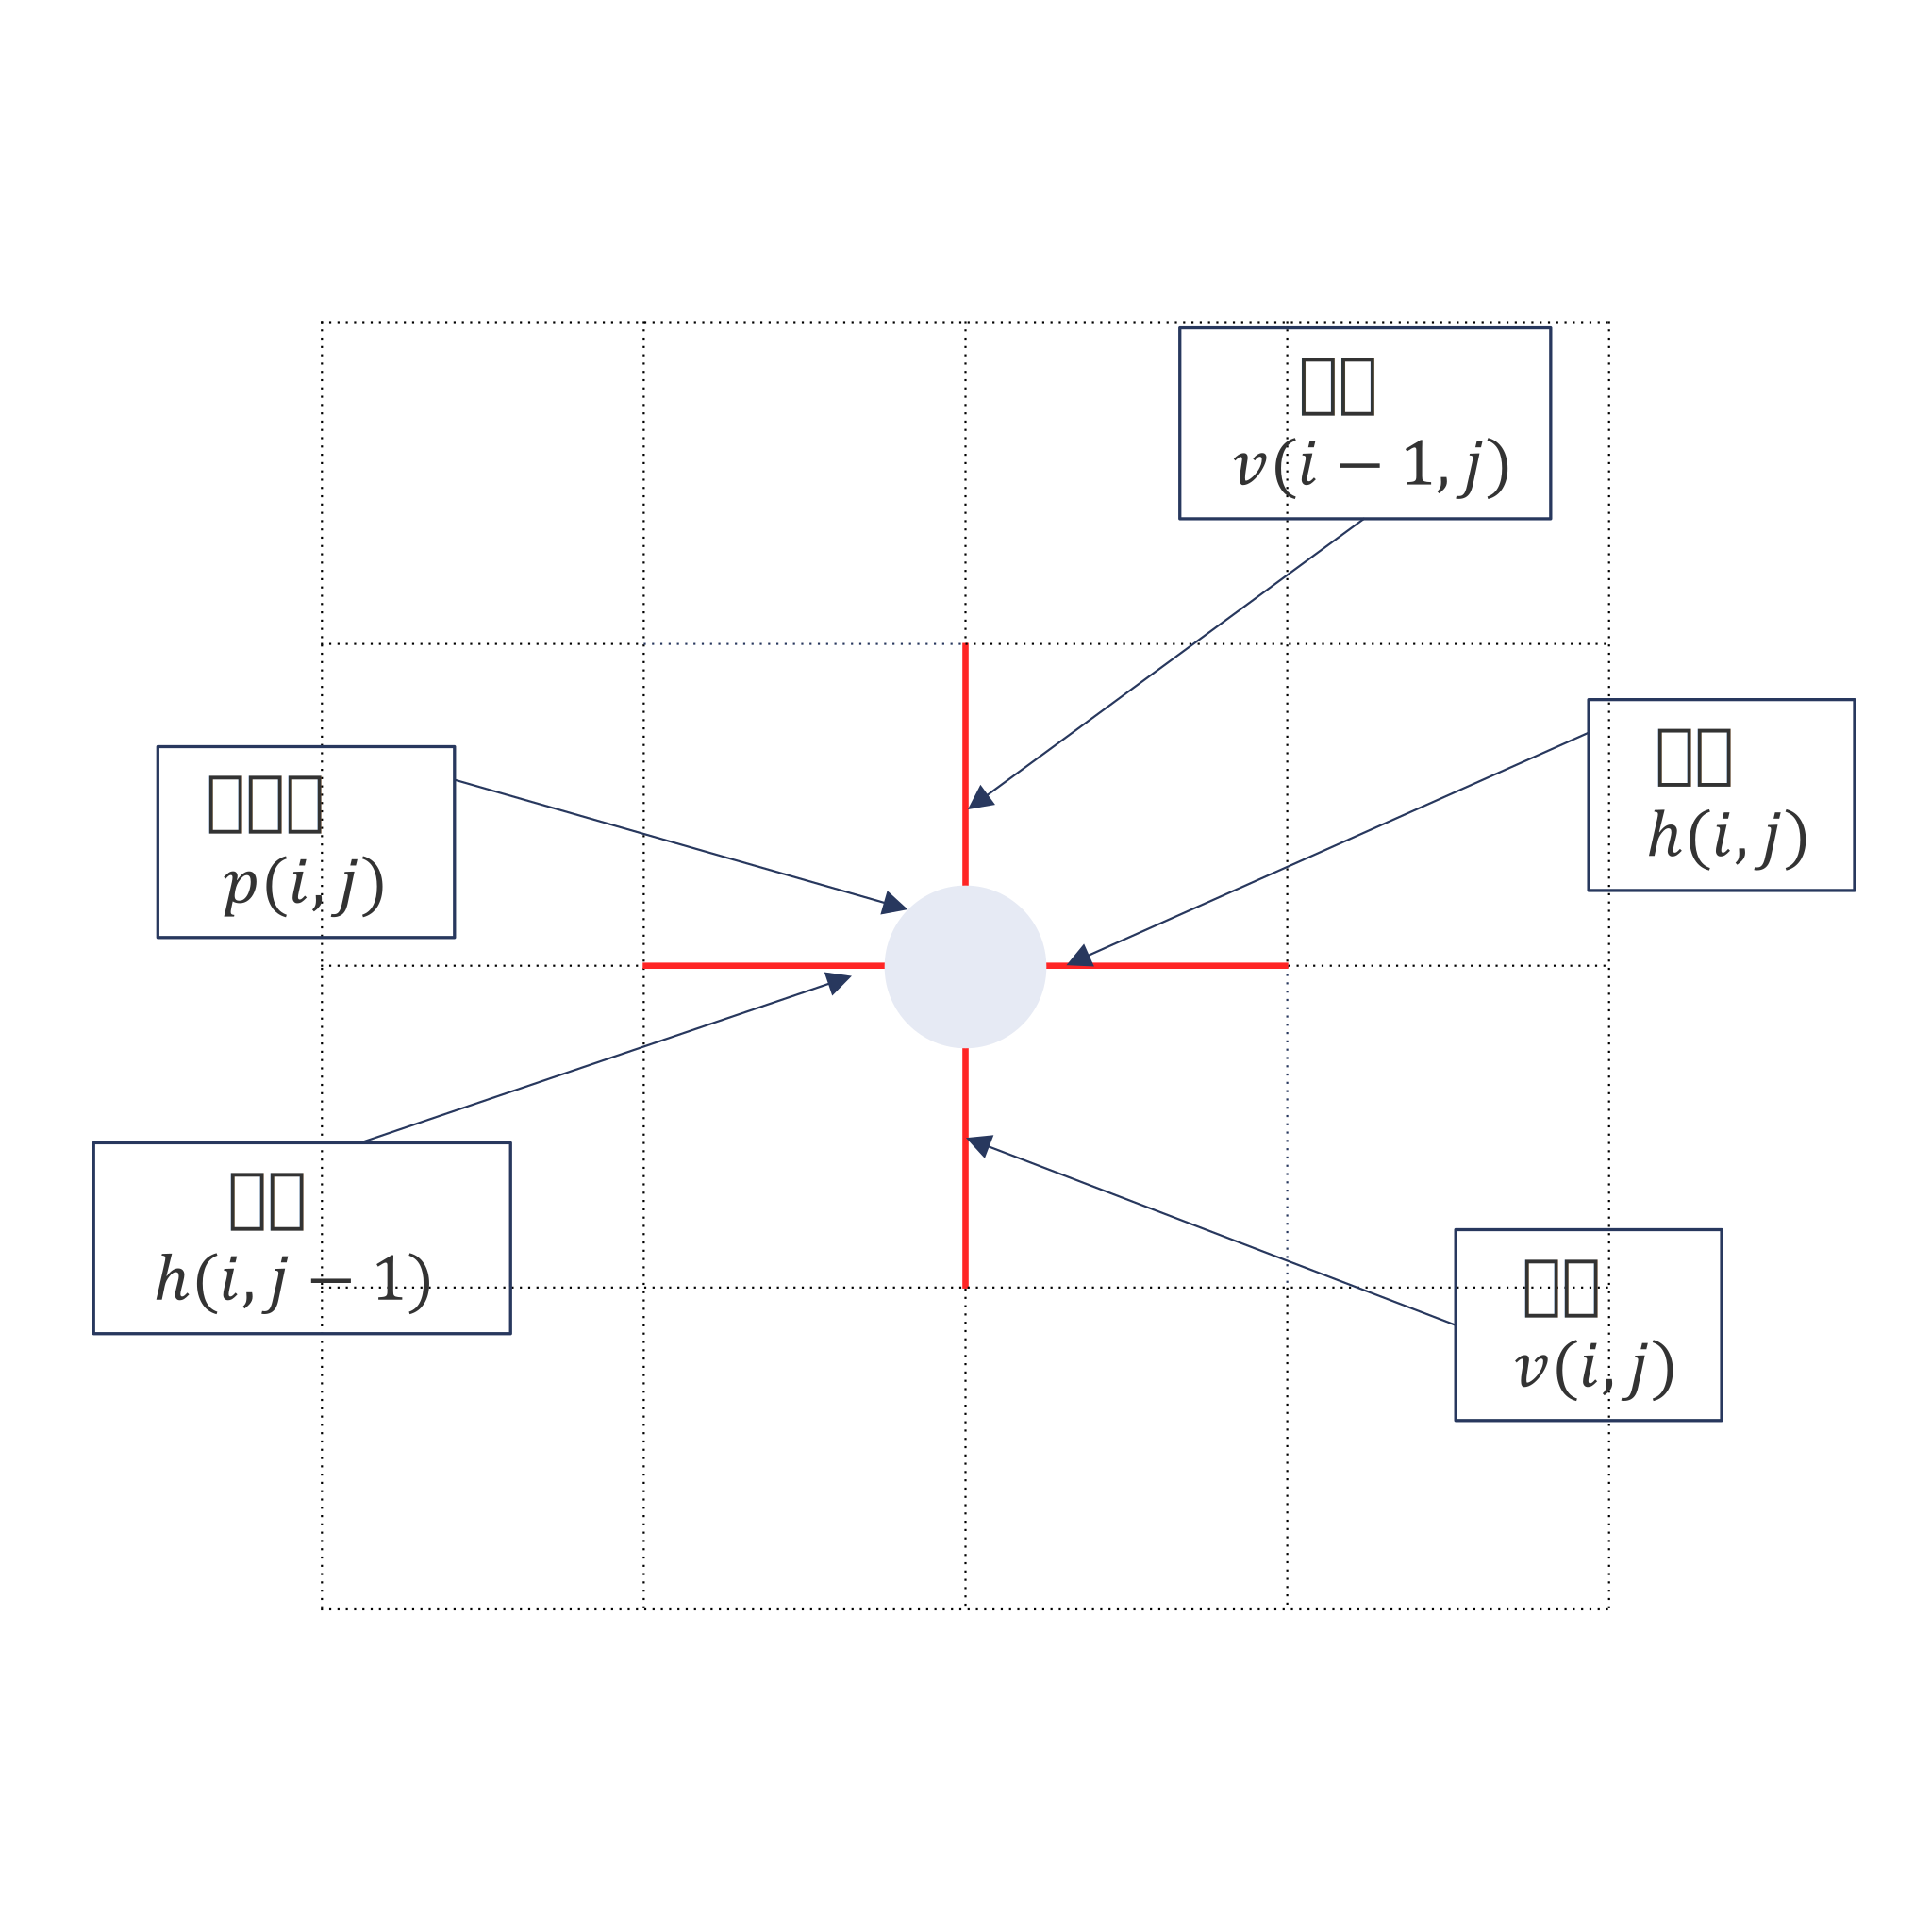
\includegraphics[width=5cm]{fig/cross.png}
  \caption{cross}
  \label{fig:cross}
\end{clearpagefigure}

\begin{clearpagefigure}
  \includegraphics[width=5cm]{fig/cycle.png}
  \caption{cycle}
  \label{fig:cycle}
\end{clearpagefigure}

\section{盤面上の変数の関係性の定義}\label{section:RelationDefinition}

次に, \cref{section:MathematicalDefinition}で定義した盤面上の変数同士の関係性について定義を行う. ただし, ここでは完成盤面を仮定する.
まず, 連結と含有, 到達可能の定義を行う.
連結とは直感的に辺と辺が繋がっていることを表す用語とし, 含有とは盤面上の変数が集合として他の変数を含むこと, 到達可能とは離れた辺と辺へと向かう道が存在することを表す用語として導入する.

\begin{definition}[連結]\label{definition:Connection}
  $e(i,j,y)$と$e(i',j',y')$が\textbf{連結}であるとは, 以下が成立することで定義する.
  \begin{gather*}
    e_{i,j,y}=1, e_{i',j',y'}  =     1          \\
    e(i,j,y)\cup e(i',j',y')  \neq  \emptyset
  \end{gather*}
\end{definition}

\begin{definition}[含有]\label{definition:Contain}
  $e(i,j,y)$が$p(i',j')$を\textbf{含む(含有する)}とは以下が成立することで定義する.
  \begin{gather*}
    e_{i,j,y}=1               \\
    e(i,j,y)\supset p(i',j')
  \end{gather*}
  以下同様に, $c(i,j)$が$e(i',j',y')$を含む, $c(i,j)$が$p(i',j')$を含むことを以下が成立することでそれぞれ定義する.
  \begin{gather*}
    e_{i',j',y'}=1             \\
    c(i,j)\supset e(i',j',y')
  \end{gather*}
  \begin{gather*}
    c(i,j)\supset p(i',j')
  \end{gather*}
\end{definition}


\begin{definition}[到達可能]
  $e(i,j,y)$と連結な$e(i_1,j_1,y_1)$, $e(i_1,j_1,y_1)$と連結な$e(i_2,j_2,y_2),...,e(i_t,j_t,y_t)$と連結な$e(i',j',y')$のような集合$\{e(i_1,j_1,y_1),e(i_2,j_2,y_2),...,e(i_t,j_t,y_t)\}$がただ一つでも存在するとき, $e(i,j,y)$から$e(i',j',y')$に\textbf{辿ることが出来る(到達可能である)}と定義する. ただし, 自分自身は常に辿ることが出来るものとする.
\end{definition}

\begin{remark}
  $e(i,j,y)$から$e(i',j',y')$に辿ることが出来る(到達可能である)ときはいつでも$e(i',j',y')$から$e(i,j,y)$に辿ることが出来る.
\end{remark}

\begin{example}[連結, 含有, 到達可能]
  \cref{fig:SamplePuzzle}において, $h(4,1)$と$v(1,4)$は連結であり, $c(3,4)$は$v(4,4)$のみを含み, $h(3,8)$から$v(8,1)$へは辿ることが出来る.
\end{example}
以上の定義を用いることによって, 新たに「線」という概念を導入することができる.

\begin{definition}[線]\label{definition:Line}
  集合$L$の全ての要素から任意の2つの元を取り出したとき, いつでもそれらが互いに辿ることができるとき集合$L$を\textbf{線}であると定義する.
\end{definition}
この線はグラフ理論の用語を用いるたときの連結グラフとほとんど同義である. \cref{fig:SamplePuzzle}において, 集合$\{h(3,2),v(4,1),h(4,1),h(5,1)\}$は線である. この線も含有という関係性を定義することができて,
\begin{definition}[線の含有]
  線$L$が線$L'$を含むとは以下が成立することで定義する.
  \begin{equation*}
    L\supset L'
  \end{equation*}
  同様に線$L$が辺$e(i,j,y)$, 格子点$p(i,j)$が含むことを以下が成立することでそれぞれ定義する.
  \begin{equation*}
    L\supset  e(i,j,y) \\
  \end{equation*}
  \begin{equation*}
    L\ni \exists e(i,j,y) \quad \mbox{s.t. $e(i,j,y)$が$p(i,j)$を含む}
  \end{equation*}
\end{definition}

\section{グラフ}\label{section:GraphDefinition}
\cref{section:RelationDefinition}で定義した概念を用いることによって, 盤面$\Bigl\{\{p_{i,j}\},\{c_{i,j}\},\{e_{i,j,y}\}\Bigr\}$を与えたとき, 盤面上にグラフという概念を導入することができる.

\begin{definition}[グラフ]\label{definition:GraphDefinition}
  グラフ$G_z$を以下で定義する.
  \begin{equation*}
    G_z=\{P_z,L_z\}=\biggl\{  \Bigl\{p(i,j)\Bigr\}_z,\Bigl\{e(i,j,y)\Bigr\}_z\biggr\}
  \end{equation*}
  ただし, $L_z$はある$e(i,j,y)$が存在したとき盤面上に存在する$e(i,j,y)$を含む線の中で集合として最大の線であり,  $P_z$は$L_z$が含む全ての$p(i,j)$の和集合とする. ただし, どの線にも含まれない$p(i,j)$もグラフと呼び, そのときに限り$G_z=\{p(i,j)\}$とし,   孤立点と呼ぶこととする($\{p(i,j)\}$は集合として, 一つの要素$p(i,j)$しか持たない集合).
\end{definition}

このようなグラフという概念が盤面に存在すると考えられ, 盤面上のグラフ全てを要素に持つ集合
\begin{equation*}
  A=\{G_1,G_2,...,G_m\}=\{G_z\}\quad (mは盤面に存在するグラフの数)
\end{equation*}
がいつでも一意に定まる. (\cref{subsection:GraphIsUniqueProof})

また, \cref{definition:Function}で取り上げた関数のうち, グラフが定義に$p(i,j)$を含むことにより$\textit{cross}$に関して「グラフ内の全ての$p(i,j)$において, $\textit{cross}(p(i,j))=2$」などという条件を構成できる. グラフという概念を導入したことにより, \cref{definition:Conditions}で取り上げた\textit{conditions}を記述することができる.
\begin{example}\textup{スリザーリンクの\textit{conditions}}\label{example:SlitherLinkConditions}
  \begin{gather*}
    B\in \forall p(i,j)   ,  \forall c_{i,j} , \textit{cross}(p(i,j))=c_{i,j} \\
    G_1\in \forall p(i,j)            , \textit{cross}(p(i,j))=2       \\
    G_xは孤立点(x\geq 2)
  \end{gather*}
\end{example}

\chapter{実証}\label{chapter:Demonstration}
\cref{chapter:Demonstration}では, \cref{chapter:Definition}で定義したパズルルールがよく定義できているか確認を行う. \cref{section:ExistsPuzzleRule}では既存のパズルルールのうち\cref{chapter:Definition}で定義したパズルルールとして説明できるものがあることを実証する. さらに\cref{section:NewPuzzleRule}ではパズルルールの自動作成の足掛けとして新しいパズルルールが作成できることを説明する.

\section{既存のパズルルール}\label{section:ExistsPuzzleRule}
今節では既存のパズルルールが\cref{chapter:Definition}で定義したパズルルールで記述できることを実証する. \textit{codomain}, HI, \textit{identification}は自明であるから\textit{conditions}と本来のパズルルールとの対応についてのみ説明を行い, 厳密な証明は省く.
実証例としてスリザーリンクとナンバーリンクを用いる. スリザーリンクのパズルルールは\cref{example:SlitherLinkRule}である. ナンバーリンクのパズルルールは以下のものである(\cite{web:NumberLink}).
\begin{example}[ナンバーリンクのパズルルール]\label{example:NumberLinkRule}\textup{}
  \begin{enumerate}
    \item 白マスに線を引いて, 同じ数字どうしをつなげましょう.\label{NumberLinkRule_1}
    \item 線は, マスの中央を通るようにタテヨコに引きます. 線を交差させたり, 枝分かれさせたりしてはいけません.\label{NumberLinkRule_2}
    \item 数字の入っているマスを通過するように線を引いてはいけません.\label{NumberLinkRule_3}
    \item 1マスに2本以上の線を引いてはいけません.\label{NumberLinkRule_4}
  \end{enumerate}
\end{example}

\begin{example}[スリザーリンクの数学的記述]
  スリザーリンクの\textit{codomain}, \textit{conditions}, HI, \textit{identification}はそれぞれ\cref{example:SlitherLinkCodomain}, \cref{example:SlitherLinkConditions}, \cref{example:SlitherLinkHiddenInformation}, \cref{example:SlitherLinkIndentification}である. \textit{conditions}に関し, \cref{example:SlitherLinkRule}の\ref{SlitherLinkRule_1}と\ref{SlitherLinkRule_3}は\cref{equation:SlitherLinkConditions_2}と\cref{equation:SlitherLinkConditions_3}に対応し, \cref{example:SlitherLinkRule}の\ref{SlitherLinkRule_2}は\cref{equation:SlitherLinkConditions_1}に対応している.

  このパズルルールから具体的に完成盤面を選んだものに\cref{figure:SlitherLink}の下図が含まれる. 非完成盤面は\cref{figure:SlitherLink}の上図であり, 確かにこれはスリザーリンクの(\cref{figure:SlitherLink}の完成盤面に対応する)問題の元であることが分かる.
\end{example}

\begin{example}[ナンバーリンクの数学的記述]
  ナンバーリンクは, 以下で示す\textit{codomain}, \textit{conditions}で定めた盤面をリプレイスすることによりナンバーリンクの盤面を表すことができる.
  \textit{codomain}は以下のように記述することができる
  \begin{align}
     & \mathbb{P}=\emptyset                                             \\
     & \mathbb{C}=\{\,\textit{null}, \emptyset ,x_1,x_2,\ldots, x_a\,\} \\
     & \mathbb{E}=\{\,\textit{null},0,1\,\}          .                  \\
  \end{align}

  \textit{conditions}は以下のように記述することができる
  \begin{align}
     & B\ni \forall p(i,j),1\le \textit{cross}(p(i,j))\le 2                          \label{equation:NumberLinkConditions_1} \\
     & B\ni \forall p(i,j), \textit{cross}(p(i,j))= 2 \Rightarrow p_{i,j}=\emptyset \label{equation:NumberLinkConditions_2}  \\
     & \forall G_z\ni P_z, |\{\,p(i,j)\mid cross(p(i,j))=1\,\}|=2             \label{equation:NumberLinkConditions_3}        \\
     & \forall G_z\ni P_z, \textit{cross}(p(i,j))= 1 \Rightarrow p_{i,j}=x_a     \label{equation:NumberLinkConditions_4} .   \\
  \end{align}

  HIは以下のように記述することができる
  \begin{equation}
    \{\,e_{i,j}\,\}.
  \end{equation}

  \textit{identification}は以下のように記述することができる
  \begin{equation}
    e:\textit{null}\leftrightarrow 0.
  \end{equation}

  \textit{conditions}に関し, \cref{example:NumberLinkRule}の\ref{NumberLinkRule_1}は\cref{equation:NumberLinkConditions_1}と\cref{equation:NumberLinkConditions_2}と\cref{equation:NumberLinkConditions_4}に含まれ, \ref{NumberLinkRule_2}は\cref{equation:NumberLinkConditions_3}に対応し, \ref{NumberLinkRule_2}は\cref{equation:NumberLinkConditions_4}に含まれ,\cref{example:NumberLinkRule}の\ref{NumberLinkRule_4}は\textit{codomain}の時点で保証される.

  このパズルルールから具体的に完成盤面を選んだものは\cref{figure:NumberLink}であり, 非完成盤面は\cref{figure:NumberLinkQuestion}であり, これをリプレイスしたものがそれぞれ\cref{figure:NumberLinkReplace}, \cref{figure:NumberLinkQuestionReplace}である. これは確かにスリザーリンクの完成盤面であることが分かる.
\end{example}

\section{新しいパズルルールの作成}\label{section:NewPuzzleRule}
\cref{section:NewPuzzleRule}では\cref{chapter:Definition}で定義したパズルルールで, 新しいパズルルールが作成できることを説明する. まず, 以下のように\textit{codomain}, \textit{conditions}, HI, \textit{identification}を次のように選ぶ.

\textit{codomain}は以下とする
\begin{align}
   & \mathbb{P}=\emptyset                       \\
   & \mathbb{C}=\{\,\textit{null},0,1,2,3,4\,\} \\
   & \mathbb{E}=\{\,\textit{null},0,1\,\}  .    \\
\end{align}
\textit{conditions}は以下とする
\begin{align}
  A\ni \forall G_z, G_z\ni L_z, |L_z|=4 \\
  B\ni \forall c(i,j), c_{i,j}= cycle(c(i,j)).
\end{align}
HIは以下とする
\begin{align}
  \{\,e(i_y,j_y,y)\,\}.
\end{align}
\textit{identification}は以下とする
\begin{align}
  e:\textit{null}\leftrightarrow 0.
\end{align}

\textit{codomain}, \textit{conditions}, HI, \textit{identification}を選んだとき, 非完成盤面と完成盤面の組み合わせとして\cref{figure:NewPuzzleRule}を考えることができる(非完成盤面であることの証明は省く).

この新しく作成したパズルルールは, 以下のように定性的に記述することができる. ただし, 以下の記述は本研究を知らなくても理解できるように, 本研究で用いた線とは違う意味で用いていることに注意する.

\begin{enumerate}
  \item 長さが4のひとつながりの線を書くこと.
  \item 各マス(細胞)の数字は周りにある辺の本数である. 例えば, 2が入っているマスの周りには2本しか辺がない.
\end{enumerate}

\begin{clearpagefigure}
  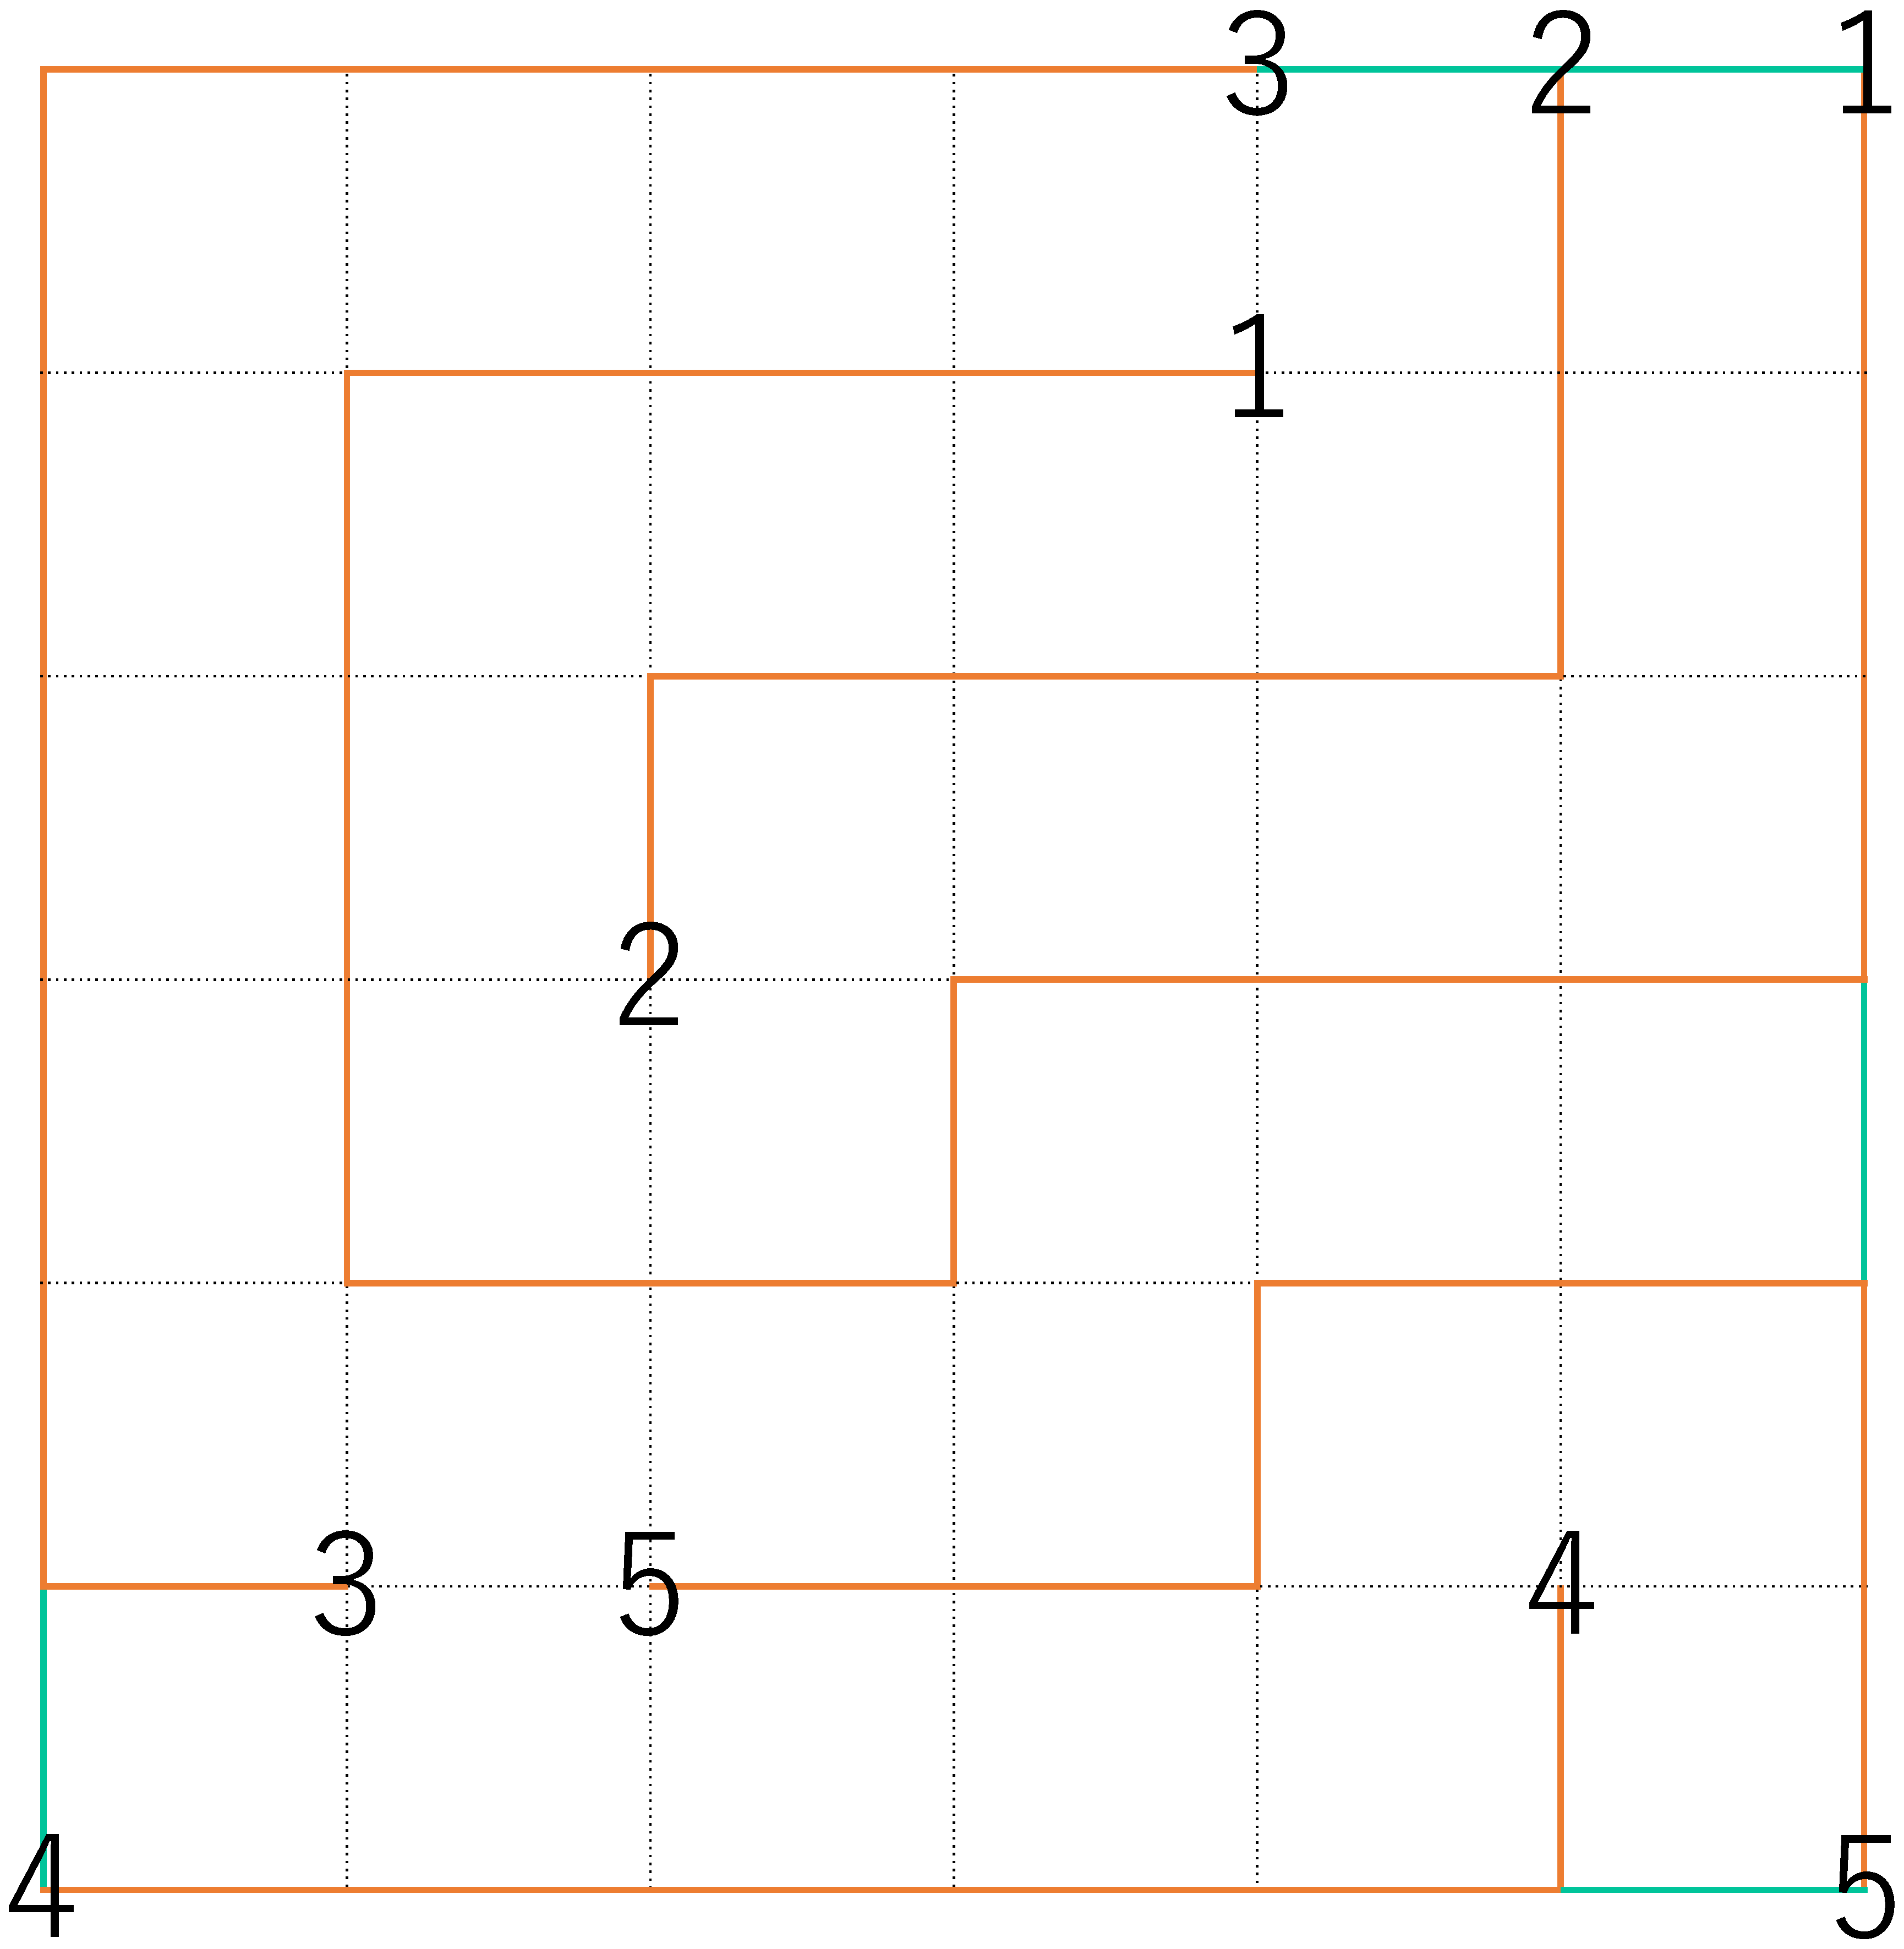
\includegraphics[width=0.85\linewidth,clip]{fig/NumberLink.eps}
  \caption{ナンバーリンクの完成盤面(リプレイス前)}
  \label{figure:NumberLink}
\end{clearpagefigure}

\begin{clearpagefigure}
  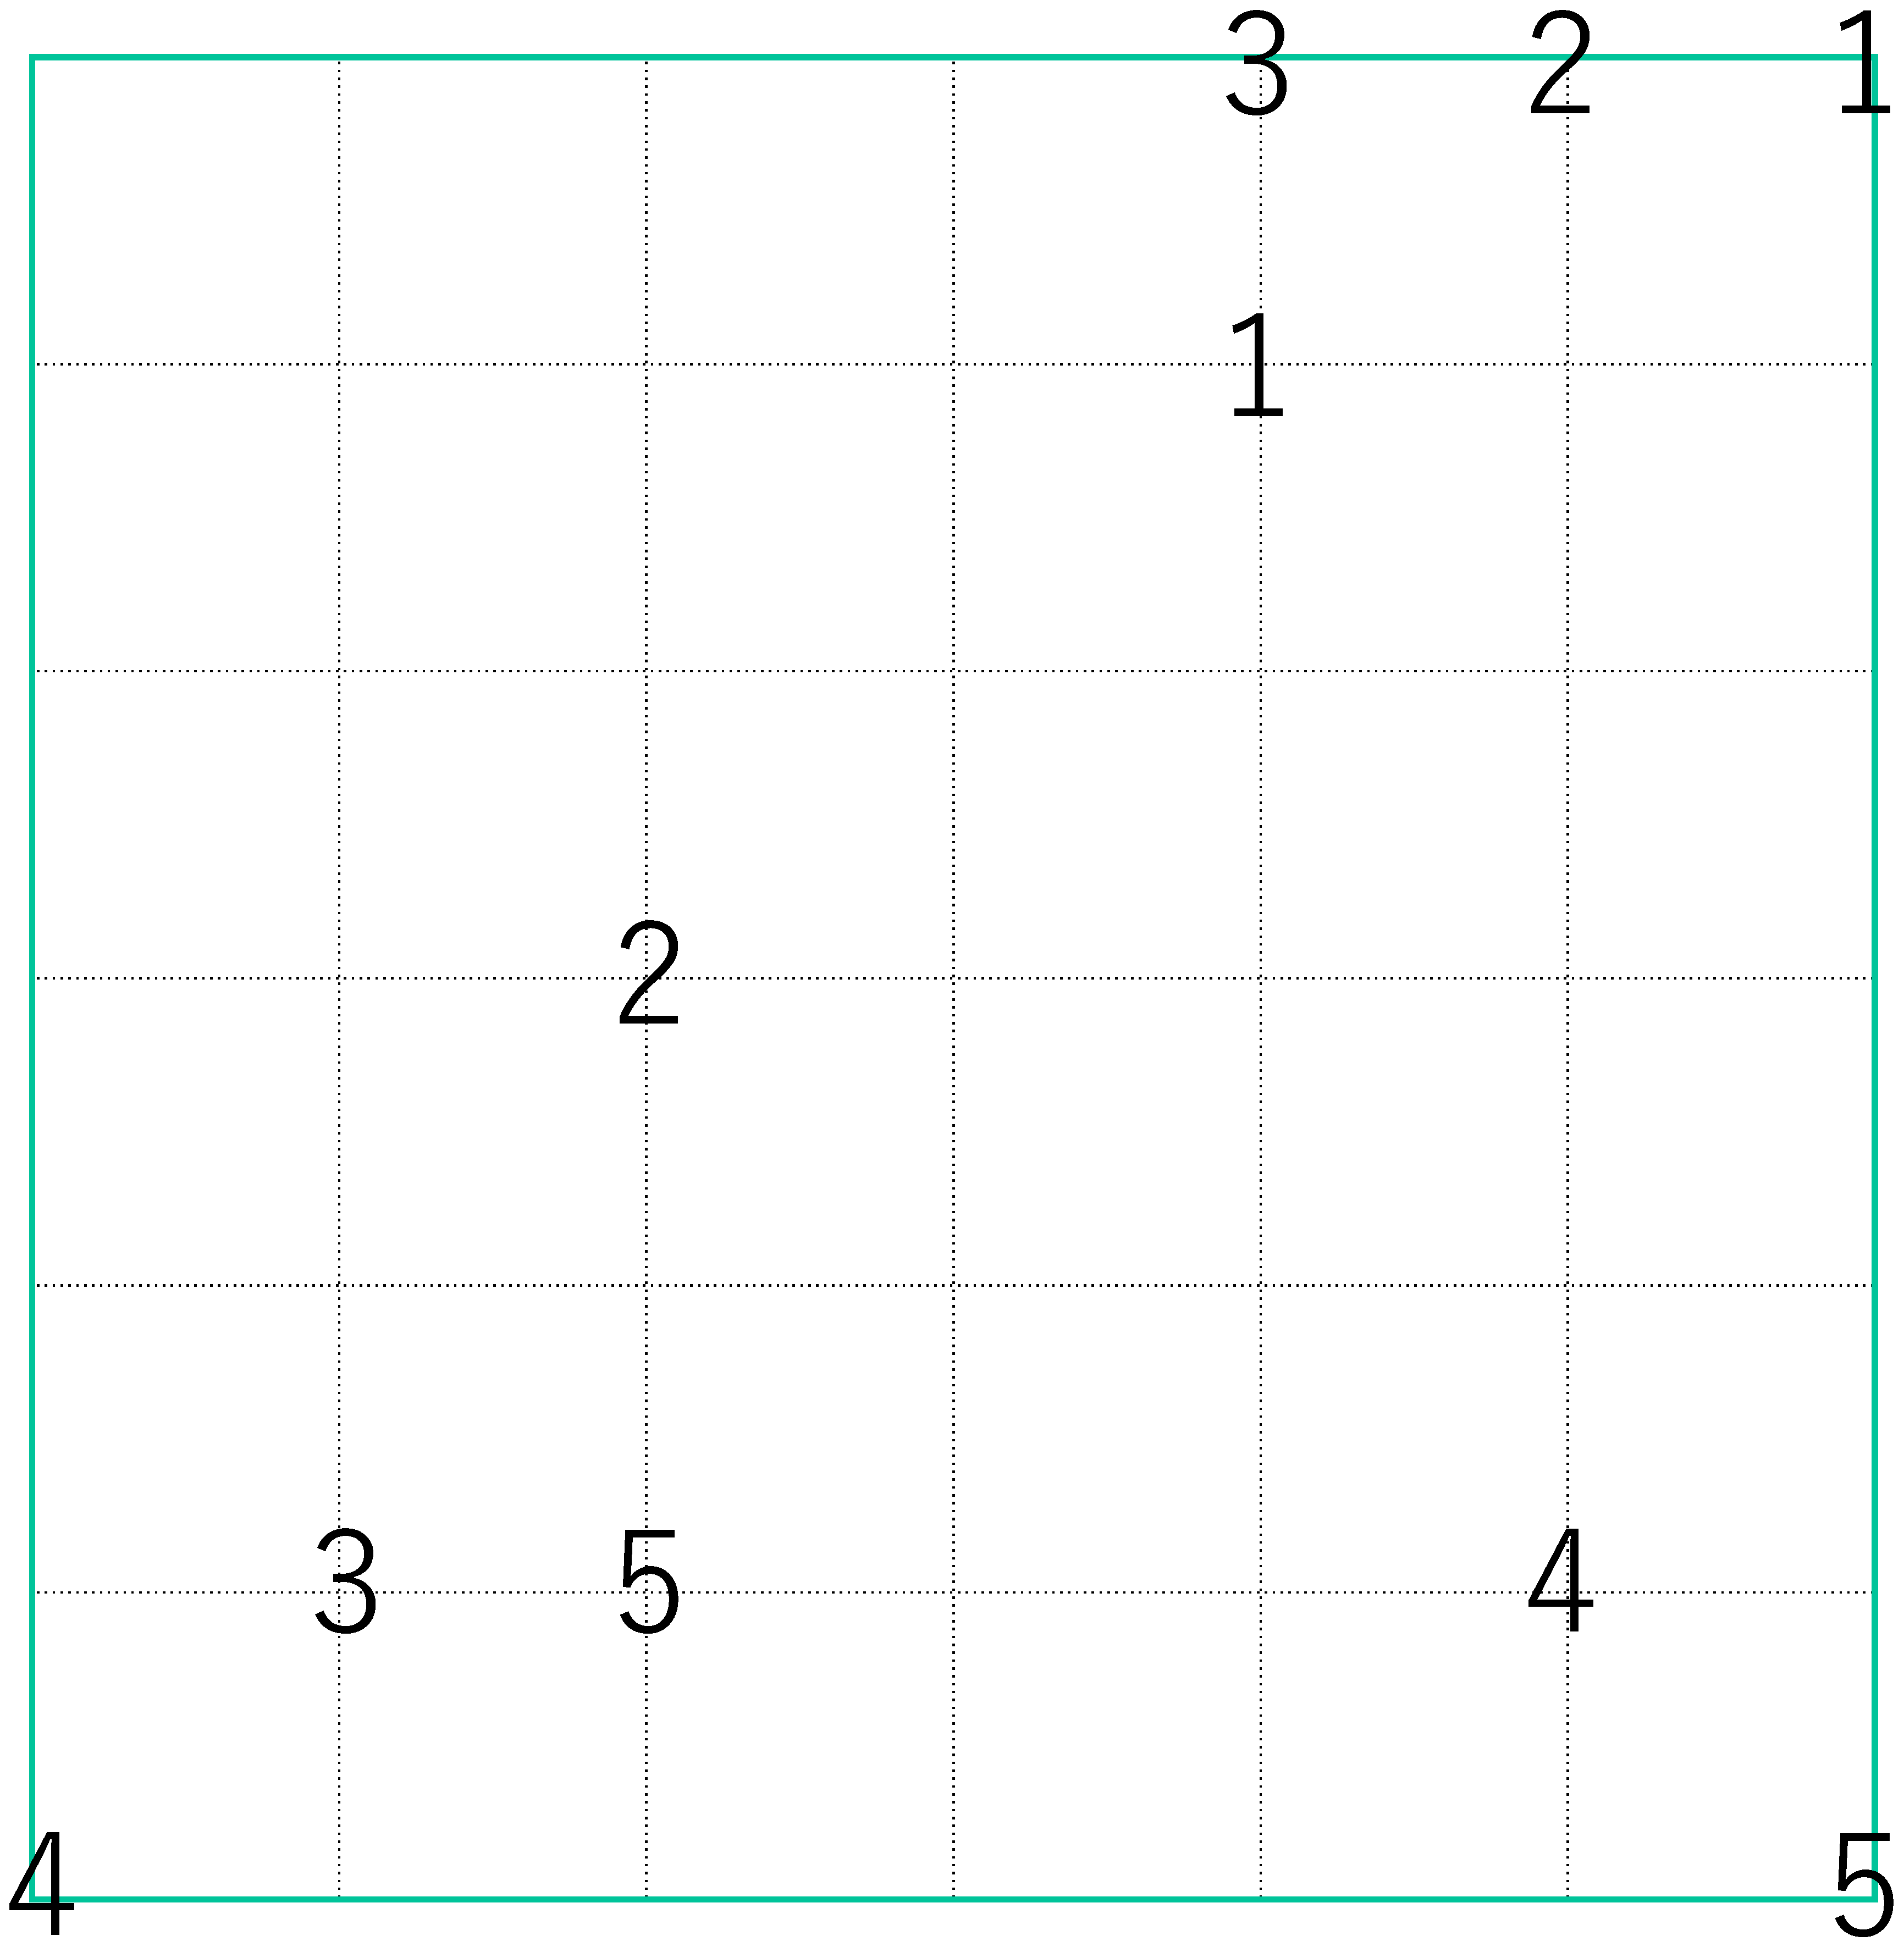
\includegraphics[width=0.85\linewidth,clip]{fig/NumberLinkQuestion.eps}
  \caption{ナンバーリンクの非完成盤面(リプレイス前)}
  \label{figure:NumberLinkQuestion}
\end{clearpagefigure}

\begin{clearpagefigure}
  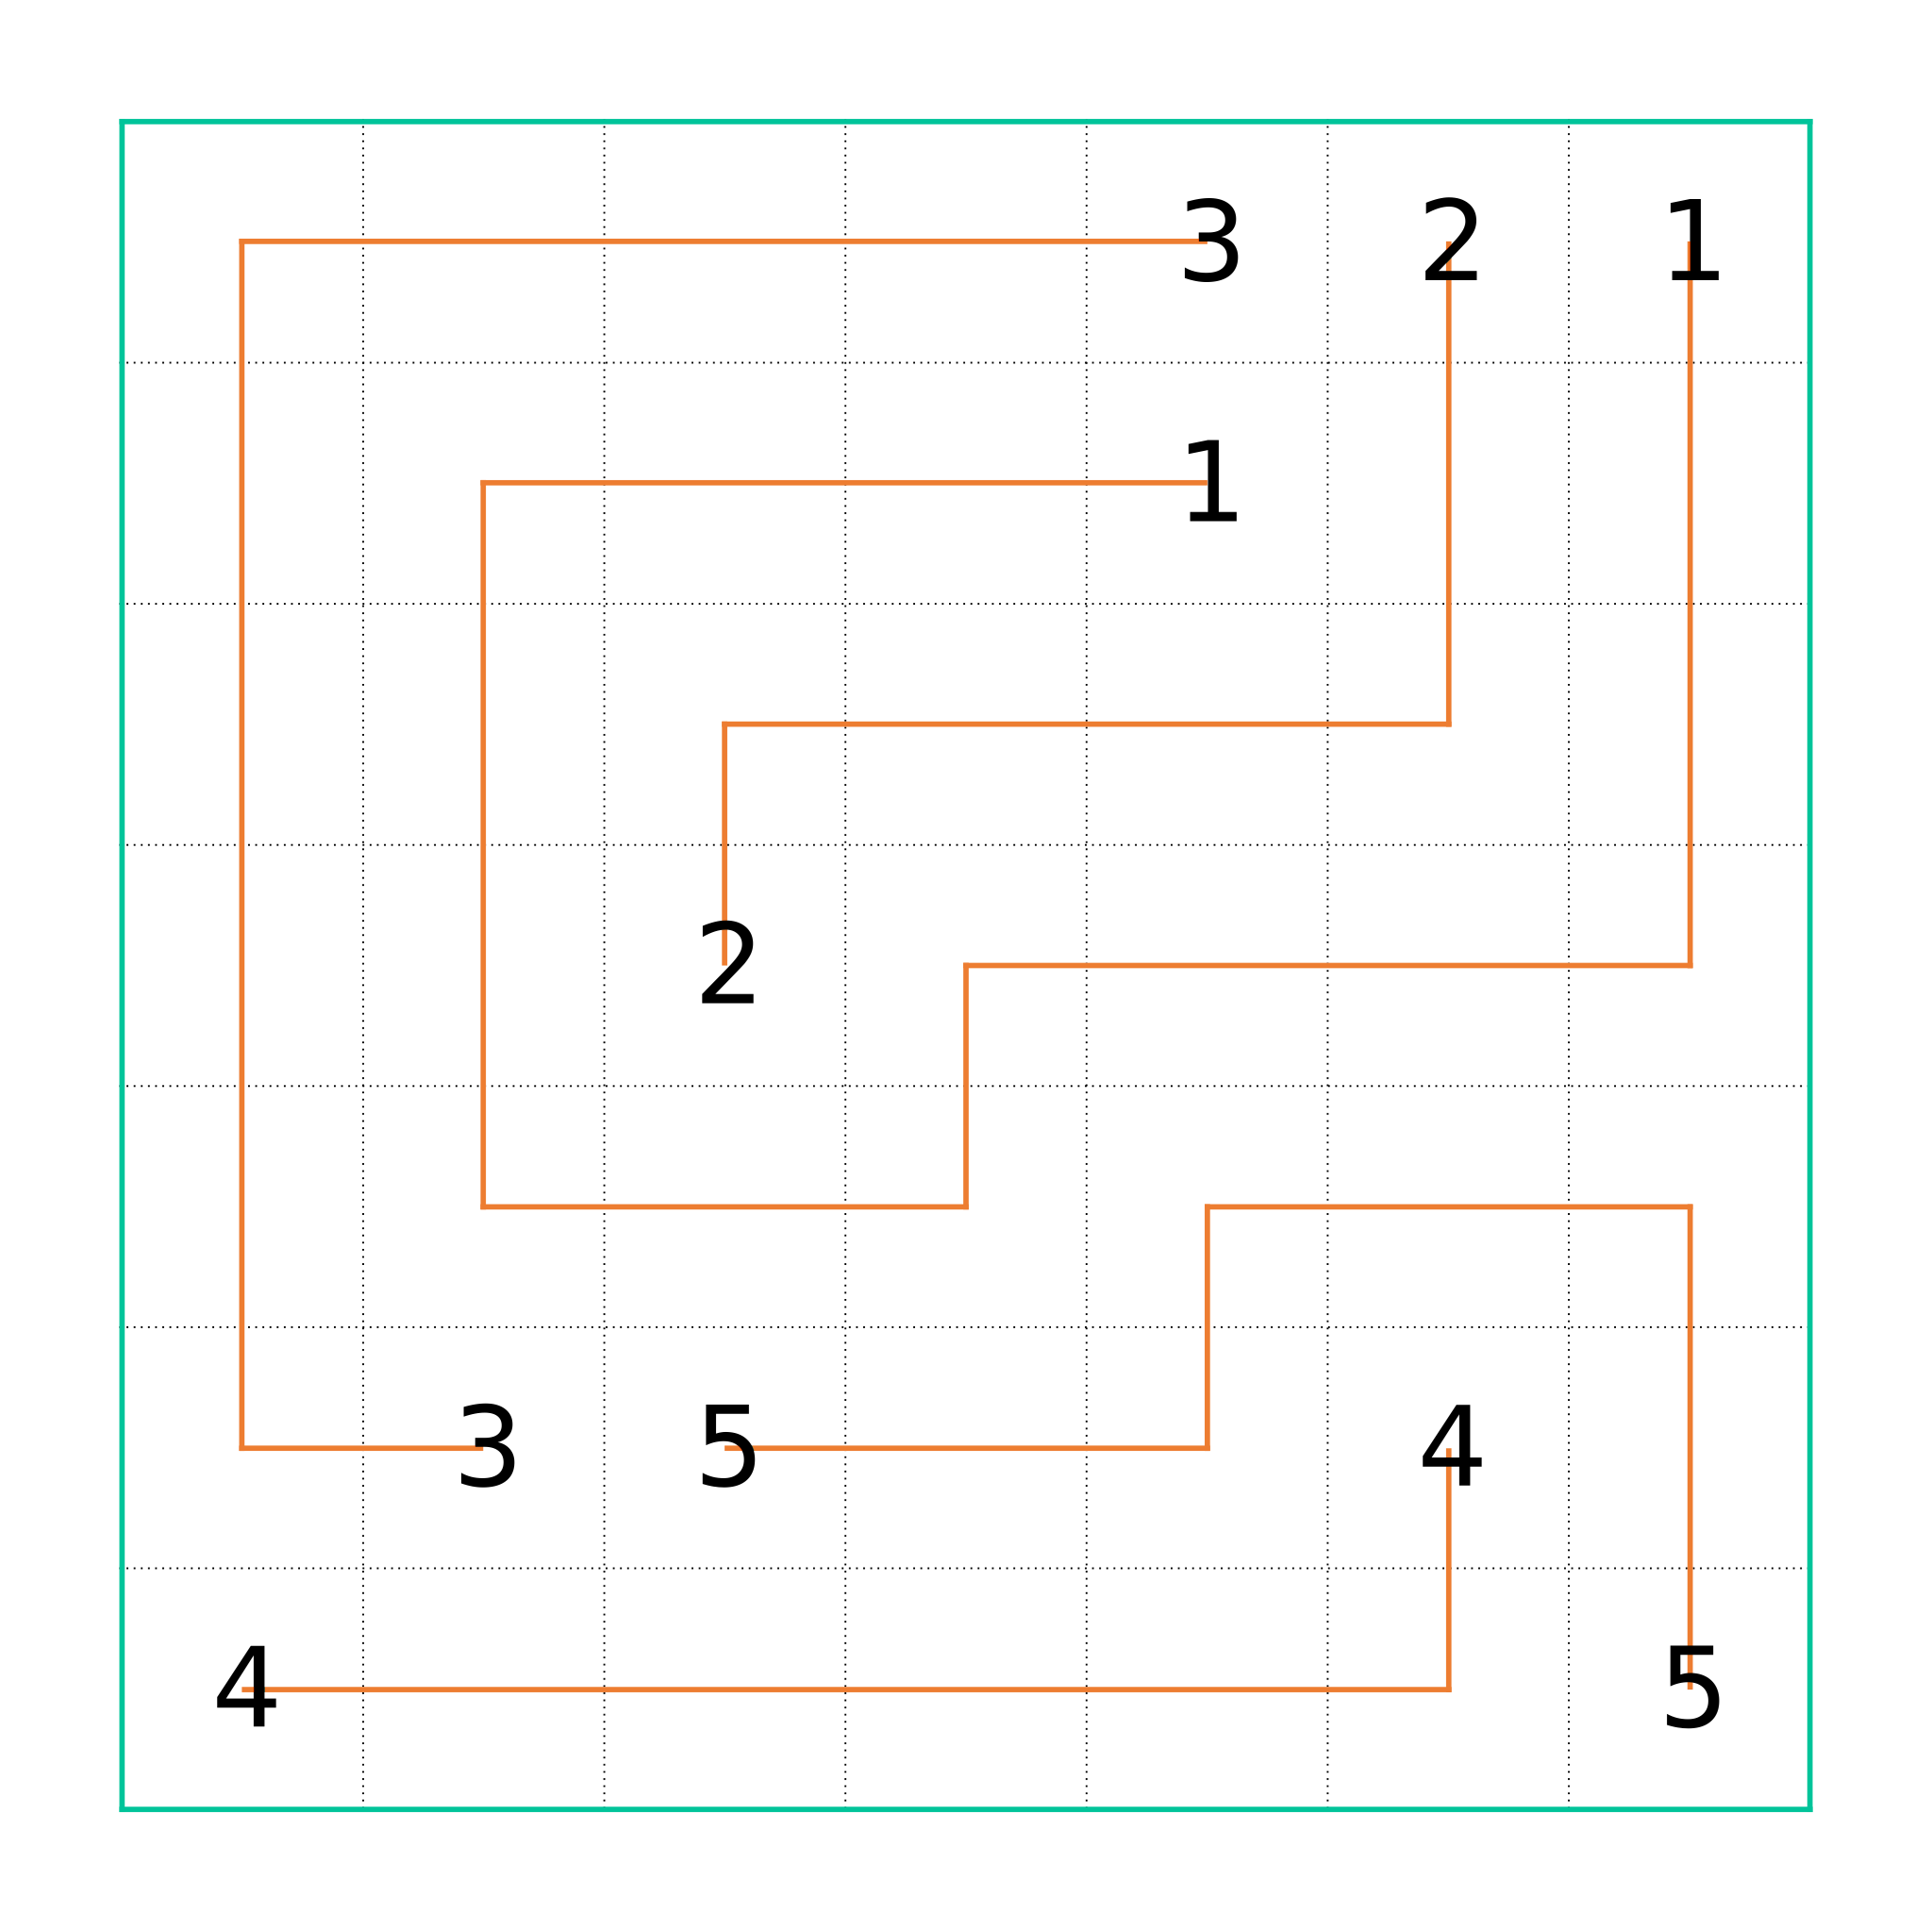
\includegraphics[width=0.85\linewidth,clip]{fig/NumberLinkReplace.eps}
  \caption{ナンバーリンクの完成盤面(リプレイス後)}
  \label{figure:NumberLinkReplace}
\end{clearpagefigure}

\begin{clearpagefigure}
  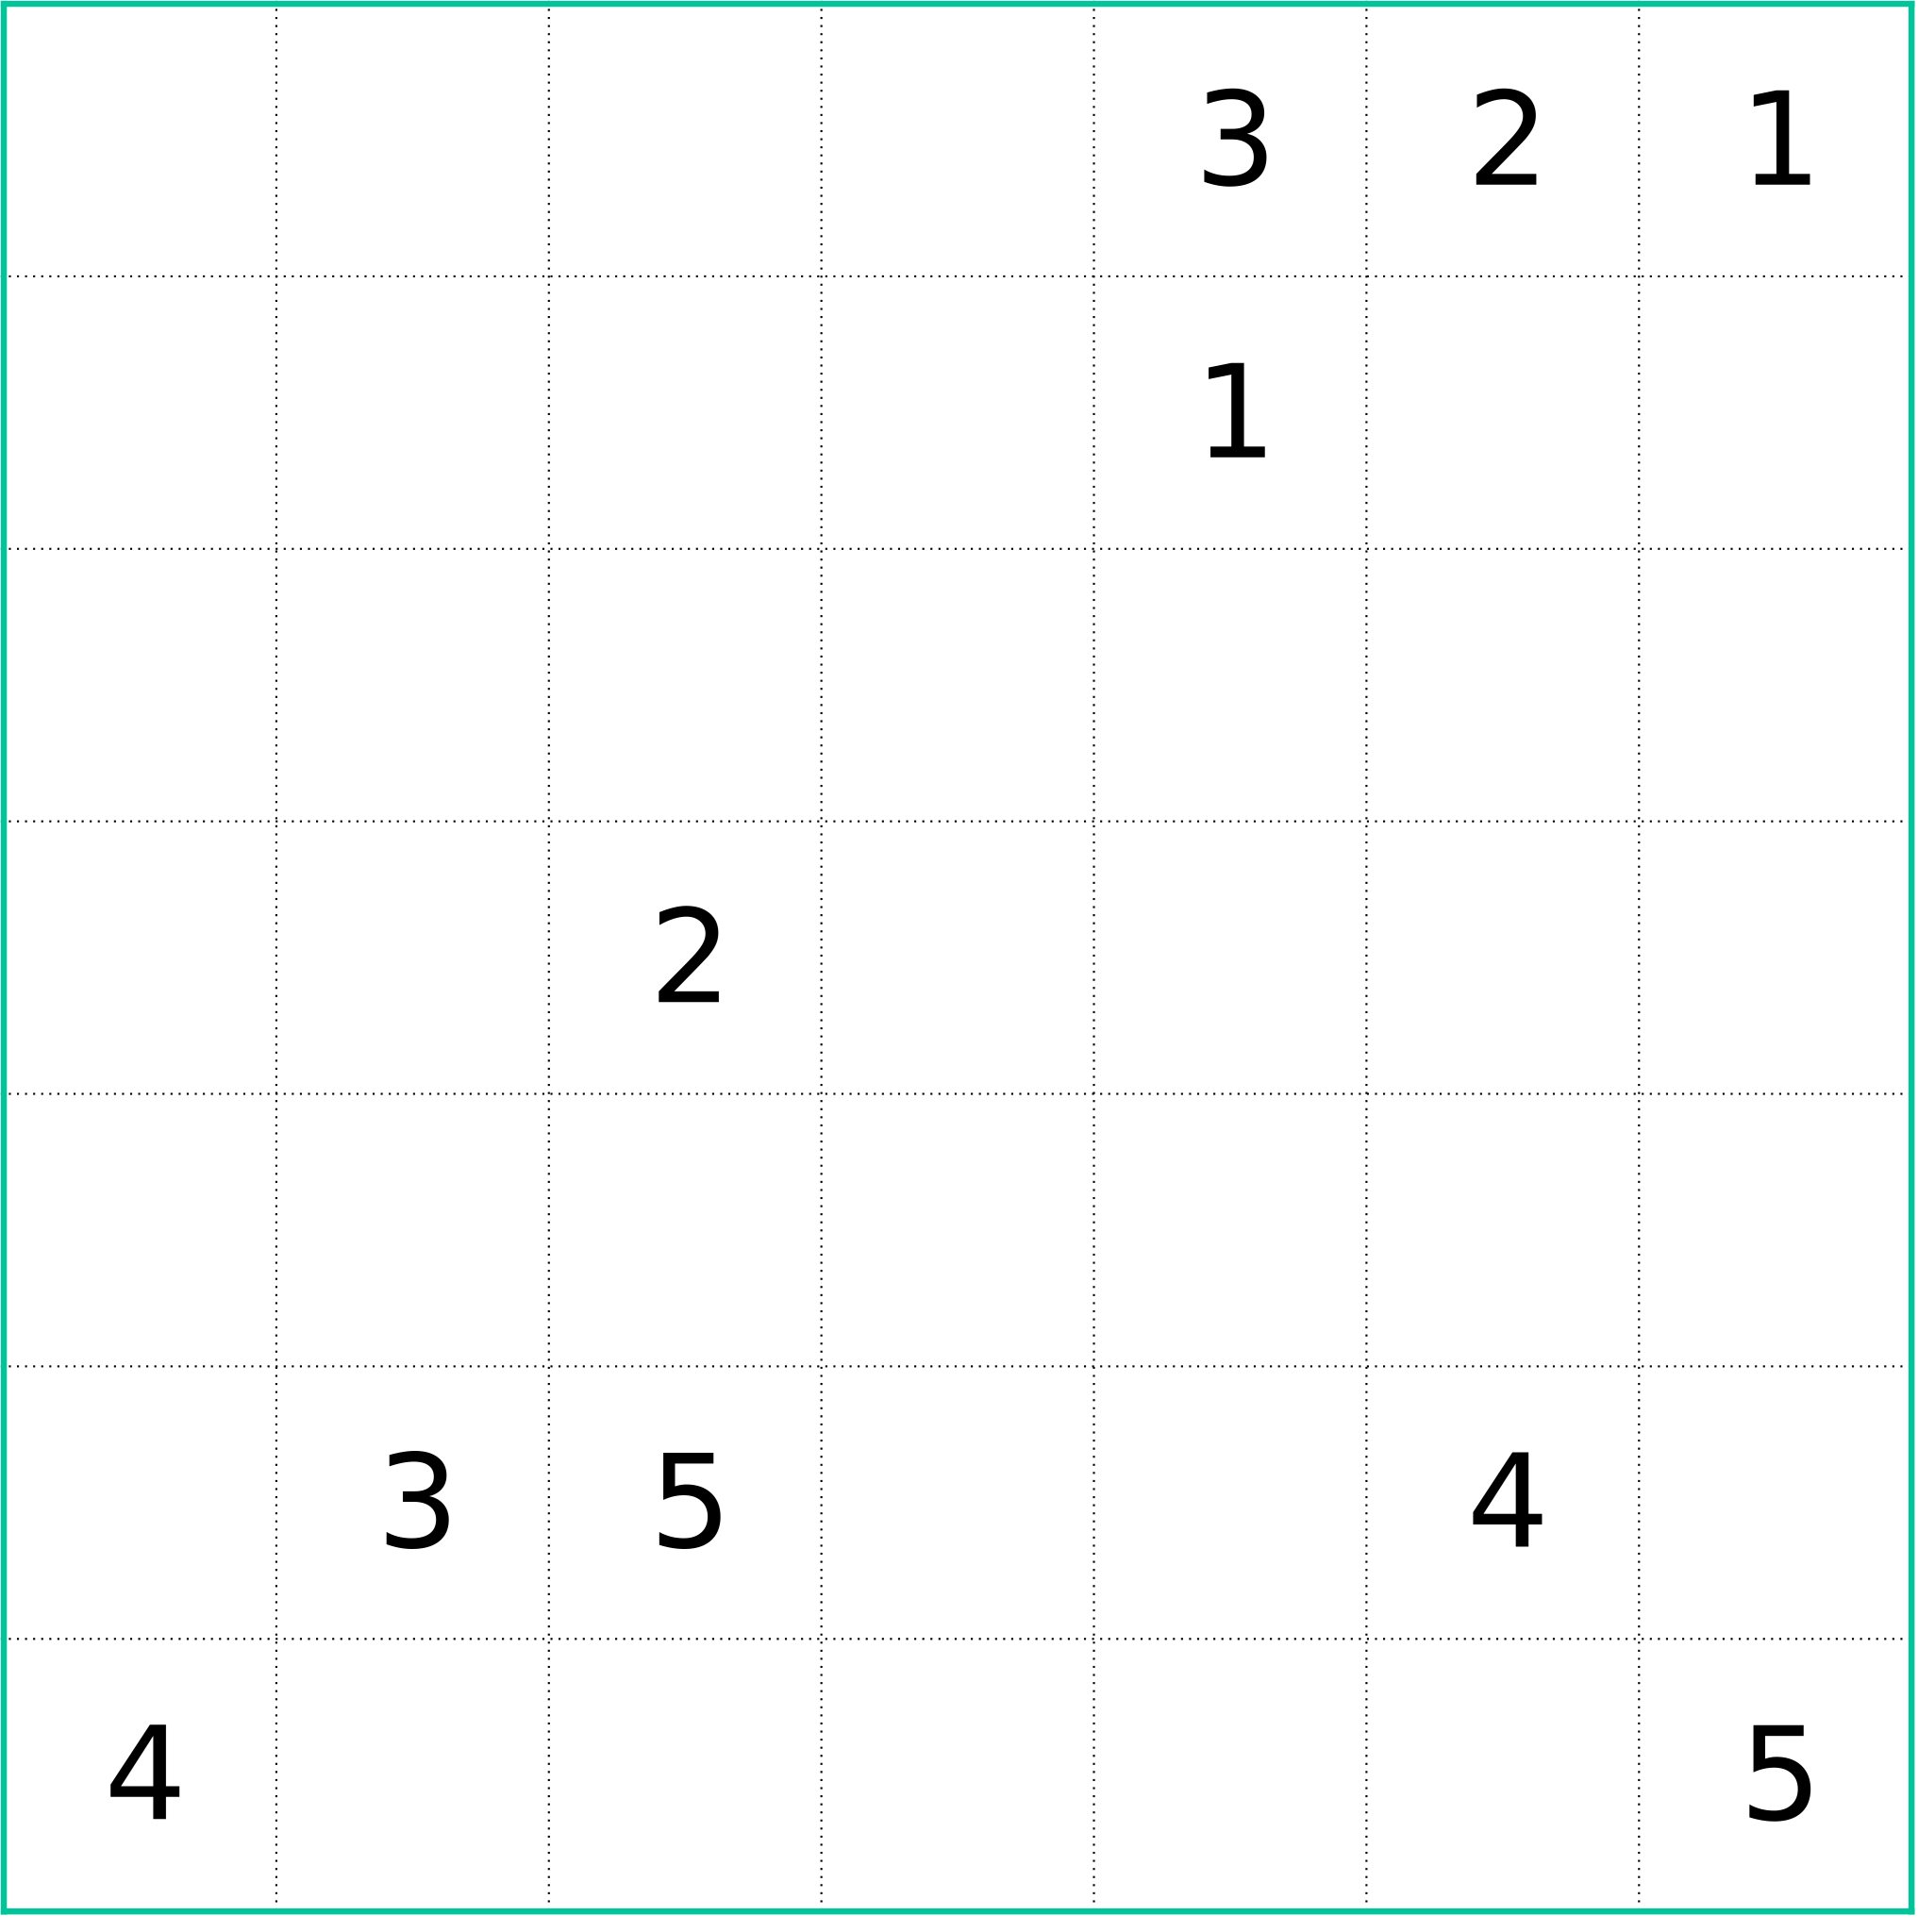
\includegraphics[width=0.85\linewidth,clip]{fig/NumberLinkQuestionReplace.eps}
  \caption{ナンバーリンクの完成盤面(リプレイス後)}
  \label{figure:NumberLinkQuestionReplace}
\end{clearpagefigure}

\begin{clearpagefigure}
  \includegraphics[width=0.5\linewidth,clip]{fig/NewPuzzleRule.eps}
  \caption{新しく作成したパズルルール. 上が非完成盤面, 下が完成盤面. }
  \label{figure:NewPuzzleRule}
\end{clearpagefigure}

\chapter{結言}
\cref{chapter:Definition}では, サイズ$m\times n$の平面グリッドを与えた際に, 種々の数学的定義を行うことでパズルルールが定義できることを主張した. また, パズルルールを構成する中枢を担う\textit{conditions}の具体的な構成方法について\cref{section:ConcreteConditions}で説明を行った. \cref{chapter:Demonstration}では本研究におけるパズルルールの定義を用いることで, 既存のパズルルールを数学的に記述することを可能にすることを示した. さらに, \cref{section:ConcreteConditions}で説明した\textit{conditions}の構成方法を用いることによって, 新規のパズルルールを作成できることを示した.

このパズルルールの定義を用いることで, 既存, 新規にかかわらずパズルルールの数学的記述ができる. さらに, \textit{conditions}の性質の分類, 抽象化を行うことでパズルルールの体系的な分類が期待される. これらが実現すればパズルルールの機械的な作成, あるいは自動作成が期待できる. 本論文中で触れた, \cref{theorem:AutoGeneration}の適用条件を明確にできれば, 自動作成したパズルルールの具体的な問題を作成できるため, 商業用ゲームへの移植が実現できる.

今後の展望として, まず本文中で触れたように\cref{theorem:AutoGeneration}の適用範囲について明確にすることが挙げられる. これに成功すれば, その適用範囲を満たしている\textit{codomain}と\textit{conditions}を満たす完成盤面を一つ考えることができれば, それは問題の存在と同値になり, より実用的になることが期待される.

さらに, ペンシルパズルの体系的な難易度評価の研究が挙げられる. 研究段階では\textit{codomain}とHIの選び方によりパズルルールの難易度が変わることが定性的に分かっている. Komiya-Kotani-Korekawa\cite{Komiya2010}はペンシルパズルの難易度を"Solution Path"という概念を考案し, 体系的に難易度評価を行っている. しかしこれはあるパズルルールが存在したときの問題の難易度であり, パズルルール自体の難易度を測る指標ではない. パズルルール自体の難易度を\textit{codomain}とHIから定量的に算出する方法があれば, 自動作成されたパズルルールがより実用的になることが期待される.

他に, ペンシルパズルの定義を本論文では平面グリッドとしたが, 実際には六角形グリッドであったり, 球体上にグリッドを配置したパズルも考えることができる. 研究段階で, 平面グリッドであるための必要十分条件が「盤面$B$において, あるグラフ$G_z$が存在したとき, $G_z \ni \forall p(i,j)$, $\text{cross}(p(i,j))\le3$」であると予想されている. この制約を外すことによって, 立体形状にグリッドを配置したパズルを体系的に考えることができると期待される.
\include{sub/chapter5}

\newcounter{pagenumberbody}
\setcounter{pagenumberbody}{\value{page}}

\appendix
\setcounter{page}{1}
\renewcommand{\thepage}{A--\arabic{page}}
\chapter{付録}
\section{ある盤面を与えたとき全てのグラフを要素に持つ集合$A$がいつでも一意に取れることの証明}\label{section:GraphUnique}
ある盤面を与えたとき, $A$(\cref{equation:A})がいつでも一意であることを証明する.
\begin{proof}
  $A=\{G_1,G_2,...,G_a\}=\{G_z\}$だが, $C=\{L_1,L_2,...,L_a\}=\{L_z\}$が一意であることを示すことと同値である. 盤面$B$を与えたとき$C$, $C'$が定まるとする. $C\ni  L_z$を取ったとき, $A'\ni  L'_{z'} \mbox{ s.t. $G_z \cap L'_{z'} \neq \emptyset $}$なる$L'_{z'}$が存在する. $L_z$, $L'_{z'}$が線であるから$L_z\cap L'_{z'}$も線である. いま, $L_z\subset L_z\cap L'_{z'}$であるが$L_z$が最大である仮定から$L_z\supset L_z\cap L'_{z'}$である. よって, $L'_{z'}$も同様の議論より, $L_z= L_z\cap L'_{z'}=L'_{z'}$である. これが$C$に含まれる線について全て成立することより, $C=C'$. $C=C'$から$A=A'$である. 以上の議論より, 題意は示された.
\end{proof}

\section{完成盤面から完成可能盤面を生成する具体的手法}\label{section:GenericAlgorithm}
藤原 \cite{Fujiwara2022}が述べた, HIを用いることにより完成盤面から完成可能盤面を生成する手法について以下で説明する. ただし, 例として藤原 \cite{Fujiwara2022}と同様に数独(ナンバープレイス)を用いる. 数独(ナンバープレイス)のパズルルールは以下のとおりである. \cite{web:Sudoku}

\begin{enumerate}
  \item あいているマスに, 1から9までの数字のどれかを入れます.
  \item タテ列 (9列あります), ヨコ列 (9列あります), 太線で囲まれた3$\times$3のブロック(それぞれ9マスあるブロックが9つあります)のどれにも1から9までの数字が1つずつ入ります.
\end{enumerate}

\begin{example}[遺伝的アルゴリズム]
  数独(ナンバープレイス)の完成盤面から完成可能盤面を生成する遺伝的アルゴリズムは以下のものである.
  \begin{enumerate}
    \item タテ列, ヨコ列, 太線で囲まれた3$\times$3のブロックの内部に数字の被りがない完成盤面$X$を1つ用意する.
    \item その盤面から, HIの具体的な位置を決め, その細胞の状態を全て$null$にする.
    \item 2. の盤面は1. の完成盤面を解として含むが, その盤面は完成可能盤面と限らない.
    \item ソルバーがその盤面を解き,
          \begin{enumerate}
            \item 唯一解であれば4. は完成可能盤面であり, 数独(ナンバープレイス)の問題である.
            \item その盤面に対応する完成盤面が存在しない, あるいは前の子孫より完成盤面が増えたらその盤面を捨てて5. へ進む(初回ならその盤面を5. へと進める. ).
            \item その盤面に対応する完成盤面が前の子孫より減ったらその盤面を採用して5. へ進む(初回ならその盤面を5. へと進める. ).
          \end{enumerate}
    \item HIの具体的な位置を変えることにより, 別の完成盤面の存在を仮定する. そのような操作を施した別の盤面を用意して4. へ戻る.
  \end{enumerate}
\end{example}

藤原 \cite{Fujiwara2022}はこの遺伝的アルゴリズムを用いて多くのペンシルパズルの問題を生成できると述べている.



\setcounter{page}{1}
\renewcommand{\thepage}{B--\arabic{page}}
\backmatter
\bibliography{reference} % reference.bibの読み込み

\chapter*{謝辞}

本研究は, 筆者が京都大学工学部物理工学科機械システム学コース在籍時に行った特別研究をまとめたものです.

京都大学工学研究科の井上康博教授・瀬波大士講師より, 多大なご指導・ご教授を賜りました. ここに謹んで感謝の意を表します. 特に, 井上康博教授からは, 指導教員として直接のご指導を賜りました. 研究のテーマを選ぶにあたり積極的にディスカッションの場を設けていただき, 無事研究として形になるようにここまでフォローアップしていただきました. 心より感謝いたします.

京都大学工学研究科マイクロエンジニアリング専攻生命数理科学分野の同期や先輩には多大なるサポートをしていただきました. 特に五十嵐康祐氏には, 研究テーマを決定するにあたり助言をいただいたほか, 本論文を完成させるにあたり少なくない回数の面談を設けていただきました. お忙しいところ時間をとっていただき, 論文として形になるまで厚くサポートしていただきました. また, 森川健太郎氏には, 研究段階から積極的に示唆を与えていただき, 筆者が行き詰らないよう, 適切にフォローしてくださいました. お二人には厚く御礼を申し上げ, 感謝いたします.

また, 兄の前田洋太博士には論文としての体裁を整えるべく, 様々なご指摘をしていただきました. この場を借りてお礼申し上げます.

末筆ではありますが, この4年間の大学生活を, 不自由なく健康で過ごせるように見守ってくれた家族に心からの感謝を表します.

\begin{flushright}
  令和4年2月\\
  前田 樹
\end{flushright}


\end{document}
